\documentclass[10pt,xcolor=table]{beamer}

\usetheme[subsectionpage=progressbar]{metropolis}

\usepackage{FiraSans}
%\setsansfont[BoldFont={FiraSans-Regular},ItalicFont={FiraSans-LightItalic},BoldItalicFont={FiraSans-Italic}]{FiraSans-Light.otf}
\usepackage{FiraMono}
%\setmonofont[BoldFont={FiraMono-Medium}]{FiraMono-Regular.otf}
\usepackage{multicol}

\setbeamertemplate{itemize subitem}{--}
\setbeamerfont{caption}{size=\footnotesize}
%\usepackage{appendixnumberbeamer}

\usepackage{listings}
\lstset{
  basicstyle=\footnotesize\ttfamily,
  backgroundcolor = \color{gray!20}
}
\lstdefinestyle{c}{language=C,
  keywordstyle=\bfseries\color{green!40!black},
  commentstyle=\itshape\color{purple!40!black},
  % identifierstyle=\color{blue},
  stringstyle=\color{orange}
}
\lstdefinestyle{shell}{language=sh,
  commentstyle=\itshape\color{purple!40!black},
  moredelim=**[is][\only<2->{\color{red}}]{@}{@},
  moredelim=**[is][\only<3>{\color{blue}}]{¿}{¿}
}
\lstdefinestyle{asm}{language=[x86masm]Assembler,
  commentstyle=\itshape\color{purple!40!black},
}
\lstdefinestyle{valgrind}{basicstyle=\footnotesize\ttfamily,
  backgroundcolor = {},
}
\usepackage{caption}
\captionsetup[lstlisting]{font={small,tt}, labelformat=empty,
  labelsep=none}

\usepackage{booktabs}
%\usepackage[scale=2]{ccicons}

\usepackage{pgfplots}
\usepgfplotslibrary{dateplot}

\usepackage{expl3}
\ExplSyntaxOn
\int_zero_new:N \g__prg_map_int
\ExplSyntaxOff
%\usepackage{tikz}
%\usetikzlibrary{tikzmark,decorations.pathreplacing,calligraphy}

% Figure's path
\graphicspath{{./figs/}}


\title{Optimization and Profiling of HPC Applications}
\subtitle{using free software resources}
\date{\today}
\author{Emilio J. Padrón González  \& Diego Andrade Canosa}
 \institute{\href{mailto:emilioj@udc.gal}{\nolinkurl{emilioj@udc.gal}} || \href{mailto:diego.andrade@udc.gal}{\nolinkurl{diego.andrade@udc.gal}}
  \\
   -- \url{http://gac.udc.es/~emilioj}||
\url{http://gac.udc.es/~diego.andrade}   
   \\Computer Architecture Group
   -- Universidade da Coruña}

\begin{document}

\maketitle

\begin{frame}{Outline}

  \setbeamertemplate{section in toc}[sections numbered]
  \tableofcontents[hideallsubsections]

\end{frame}




\section{Introduction}

\frame{
  \frametitle{Paraver et al: an overview of BSC Performance Tools}
  % \item ompP
  \begin{block}{Leveraging BSC's HPC Performance
      Tools~\footnote{Barcelona Supercomputing Center Performance
        Tools: \url{http://tools.bsc.es}\\~~~Repositories:
        \url{http://github.com/bsc-performance-tools}} to profile and
      optimize parallel applications}
    \begin{center}
      Basic toolchain:~~~~~~~~~~~~~~~~~~~~~~~~~~~~~~~~~~~~~~~~~~~~~~~~~~~~~~~~~~~~~~~~~
    \item Extrae $\Rightarrow$ Paraver $\Rightarrow$ Dimemas
    \end{center}
  \end{block}

  \begin{description}
  \item[Extrae:] package that generates Paraver-trace files for
    a post-morten analysis
  \item[Paraver:] trace visualization and analysis browser
  \item[Dimemas:] high-abstracted network simulator for message-passing programs
  \end{description}
}

\frame{
  \frametitle{BSC's performance analysis tools}

  Let's embrace again this \underline{core idea} (from a previous slide):

  \begin{block}{}
    \begin{quotation}
      Profile first, optimize later
    \end{quotation}
  \end{block}

  \begin{itemize}
  \item Analysis must be the first step towards the optimization of an
    application
  \item Performance analysis tools allow us to identify and
    characterize the inefficiencies that cause a poor performance
  \end{itemize}

  \pause

  \begin{block}{BSC's toolchain main objectives:}
    \begin{itemize}
    \item flexibility and versatility: platforms, environments,
      programming models\ldots
    \item simplify and facilitate the process of extracting information from the performance data
    \end{itemize}
  \end{block}
}



\section{Dynamic instrumentation to trace programs with {\tt extrae}}

\frame{
  \frametitle{Extrae}

  {\bf Extrae}: dynamic instrumentation package to trace programs
  \begin{itemize}
  \item Generates trace files that can be later visualized with {\bf
      Paraver}
  \item Works with different programming models:
    \begin{itemize}
    \item shared memory model (such as OpenMP and pthreads)
    \item the message passing (MPI)
    \item hybrid
    \end{itemize}
  \end{itemize}
}

\frame{
  \frametitle{Extrae: main features}

  \begin{itemize}
  \item Parallel programming models \tikzmark{start}
    \begin{itemize}
    \item MPI, OpenMP, pthreads, OmpSs, CUDA, OpenCL,\\ Java, Python\ldots
    \end{itemize}
  \item Platforms
    \begin{itemize}
    \item Intel, Cray, BlueGene, MIC, ARM, Android,\\ Fujitsu Spark\ldots
    \end{itemize}
  \item Hardware Performance Counters
    \begin{itemize}
    \item Using PAPI interface
    \end{itemize}
  \item Link to source code
    \begin{itemize}
    \item Callstack at MPI routines
    \item OpenMP outlined routines
    \item Selected user functions (Dyninst)
    \end{itemize}
  \item Periodic sampling \tikzmark{end}
  \item User events (Extrae API)
  \end{itemize}

  \begin{tikzpicture}[remember picture,overlay]
    \draw[decorate,decoration={calligraphic brace}]
    ([yshift=10pt,xshift=150pt]{{pic cs:end}|-{pic cs:start}}) --
    node[xshift=5pt,anchor=west] {\parbox{5cm}{No need to\\ recompile/link!}}
    ([xshift=150pt]{pic cs:end})
    ;
  \end{tikzpicture}
}

\frame{
  \frametitle{Extrae: how it works}

  \begin{itemize}
  \item Symbol substitution through LD\_PRELOAD \hfill \alert{\bf $\leftarrow$ Recommended!}
    \begin{itemize}
    \item Specific \underline{tracing libraries} for each combination of runtimes
      \begin{itemize}
      \item MPI
      \item OpenMP
      \item OpenMP+MPI
      \item \ldots
      \end{itemize}
    \end{itemize}
  \item Dynamic instrumentation
    \begin{itemize}
    \item Based on DynInst (developed by U.Wisconsin/U.Maryland)
      \begin{itemize}
      \item Instrumentation in memory
      \item Binary rewriting
      \end{itemize}
    \end{itemize}
  \item Alternatives
    \begin{itemize}
    \item Static link (i.e., PMPI, Extrae API)
    \end{itemize}
  \end{itemize}
}

\frame{
  \frametitle{Extrae: typical scenario}

  \begin{itemize}
  \item Traces are obtained with {\bf Extrae} in a Supercomputer
    running the code to optimize:
    \begin{itemize}
    \item using the {\tt LD\_PRELOAD} mechanism to intercept entries and
      exits to MPI
    \item data from hardware counters (cache misses, instructions and
      cycles) at those points
    \end{itemize}
  \item Traces are analysed post-mortem in a PC with {\bf Paraver},
    and maybe also with {\bf Dimemas}
  \item Batch analysis possibility: {\bf Paramedir}
  \end{itemize}
}

\frame{
  \frametitle{Extrae: how to use it}

  In a nutshell:
  \begin{enumerate}
  \item Adapt the job submission script
  \item \structure{[optional]} Tune the Extrae XML configuration file
    \begin{itemize}
    \item Examples distributed with Extrae:\\
      \hfill {\footnotesize \tt \$\{EXTRAE\_HOME\}/share/example}~\footnote{In
        Finisterrae II:\\~~~{\scriptsize
          EXTRAE\_HOME=/opt/cesga/easybuild-cesga/software/MPI/gcc/6.4.0/openmpi/2.1.1/extrae/3.5.2}}
    \end{itemize}
  \item Submit/Run the job to generate the trace
  \end{enumerate}

  \pause

  All details in Extrae official documentation:
  {\small \url{https://tools.bsc.es/sites/default/files/documentation/pdf/extrae-3.5.2-user-guide.pdf}}
}



\begin{frame}[fragile]{Extrae: submission script}

  \vspace*{-0.8cm}
  \begin{lstlisting}[style=shell,gobble=3,caption={submit\_trace.sh}]
    #!/bin/sh
    #SBATCH -t 00:20:00 # execution time hh:mm:ss *OB*
    #SBATCH -n 16 #tasks (MPI processes)
    #SBATCH -c 24 #cores/task (shared-mem threads/process)
    ##SBATCH -N 16  #nodes
    #SBATCH -p cola-corta

    @module load gcc/6.4.0 openmpi/2.1.1 extrae/3.5.2
    # export TRACE_NAME=trace_filename.prv # *OP*
    @
    srun -n 16 @${HOME}/trace.sh@ parallel_binary [params]
  \end{lstlisting}

  \pause

  \vspace*{-0.8cm}
  \begin{lstlisting}[style=shell,gobble=3,caption={trace.sh}]
    #!/bin/sh
    source /opt/cesga/easybuild-cesga/software/MPI/gcc/6.4.0\
                    /openmpi/2.1.1/extrae/3.5.2/etc/extrae.sh
    ¿export EXTRAE_CONFIG_FILE=${HOME}/extrae.xml¿
    ¿export LD_PRELOAD=${EXTRAE_HOME}/lib/libmpitrace.so¿ # C code

    $*     # Run the program
  \end{lstlisting}
\end{frame}

\frame{
  \frametitle{Extrae: tracing library to use}

  \begin{table}
    \caption{Tracing libraries~\footnote{Include suffix `f' for Fortran
        codes} to use with {\tt LD\_PRELOAD}}
    \rowcolors{2}{}{gray!20}
    \begin{tabular}{lccccc}
      {\bf Library} & {\bf Serial} & {\bf MPI} & {\bf OpenMP} & {\bf pthreads} & {\bf CUDA}\\
      libseqtrace & \structure{\checkmark} & & & & \\
      libmpitrace[f] & & \structure{\checkmark} & & & \\
      libomptrace & & & \structure{\checkmark} & & \\
      libpttrace & & & & \structure{\checkmark} & \\
      libcudatrace & & & & & \structure{\checkmark}\\
      libompitrace[f] & & \structure{\checkmark} & \structure{\checkmark} & & \\
      libptmpitrace[f] & & \structure{\checkmark} & & \structure{\checkmark} & \\
      libcudampitrace[f] & & \structure{\checkmark} & & & \structure{\checkmark}\\
    \end{tabular}
  \end{table}
}

\frame{
  \frametitle{Extrae: XML configuration}

  See examples in {\tt \$\{EXTRAE\_HOME\}/share/example}

  For example:
  \begin{itemize}
  \item for MPI + OpenMP:\\
    {\tt \$\{EXTRAE\_HOME\}/share/example/MPI+OMP/extrae.xml}
  \item only MPI:\\
    {\tt \$\{EXTRAE\_HOME\}/share/example/MPI/extrae.xml}
  \item only OpenMP:\\
    {\tt \$\{EXTRAE\_HOME\}/share/example/OMP/extrae.xml}
  \end{itemize}
}

\frame{
  \frametitle{Extrae: XML configuration, easy to customize (i)}

  \begin{figure}
    \hspace*{-0.5cm}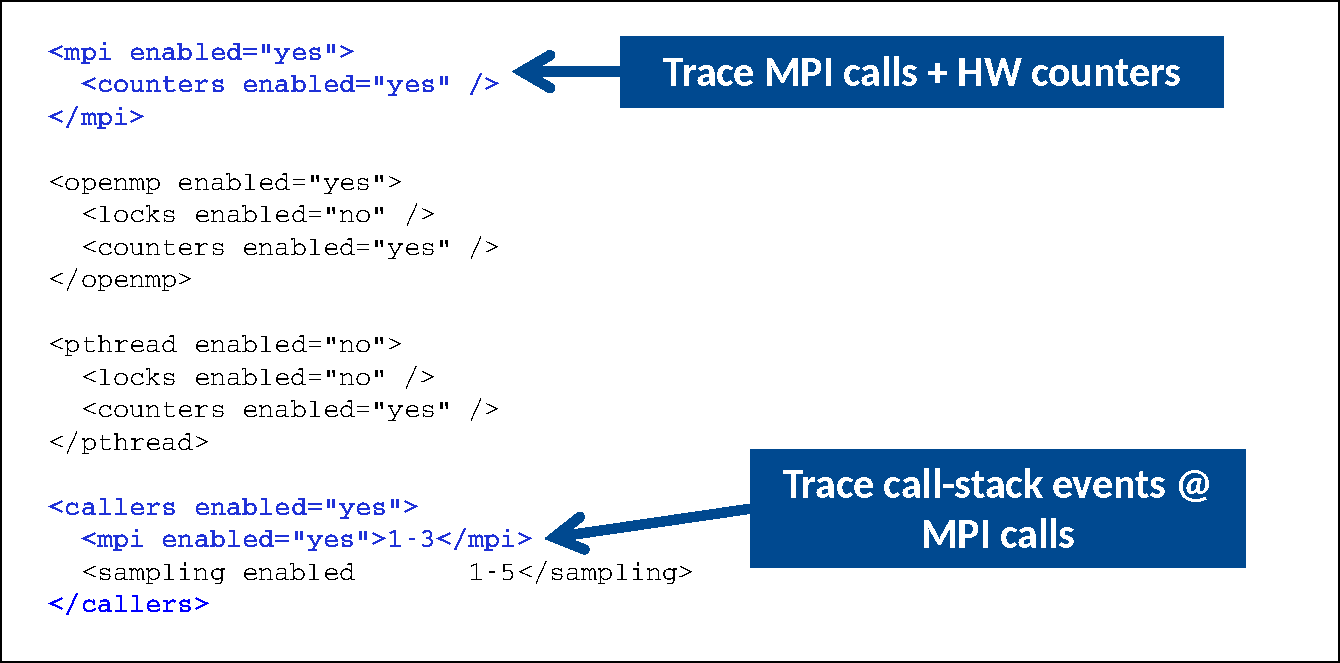
\includegraphics[width=1.1\textwidth]{extraexml1}
  \end{figure}
}

\frame{
  \frametitle{Extrae: XML configuration, easy to customize (ii)}

  \begin{figure}
    \hspace*{-.8cm}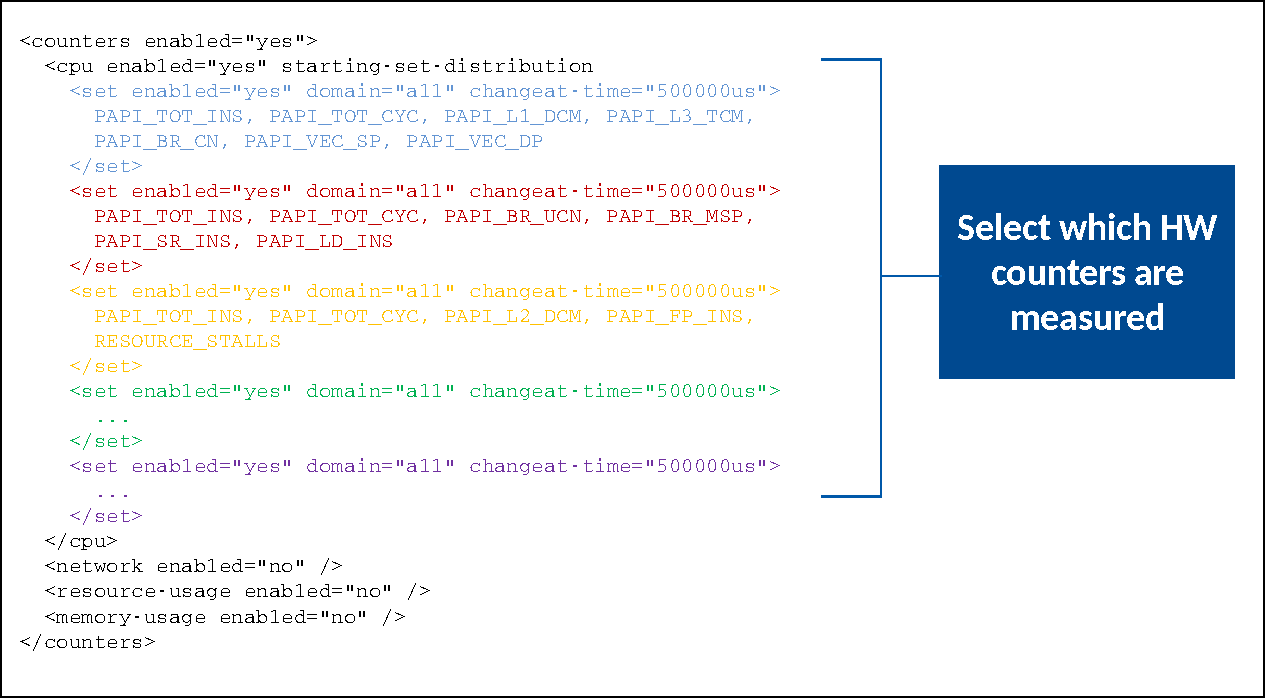
\includegraphics[width=1.15\textwidth]{extraexml2}
  \end{figure}
}

\frame{
  \frametitle{Extrae: XML configuration, easy to customize (iii)}

  \begin{figure}
    \hspace*{-0.5cm}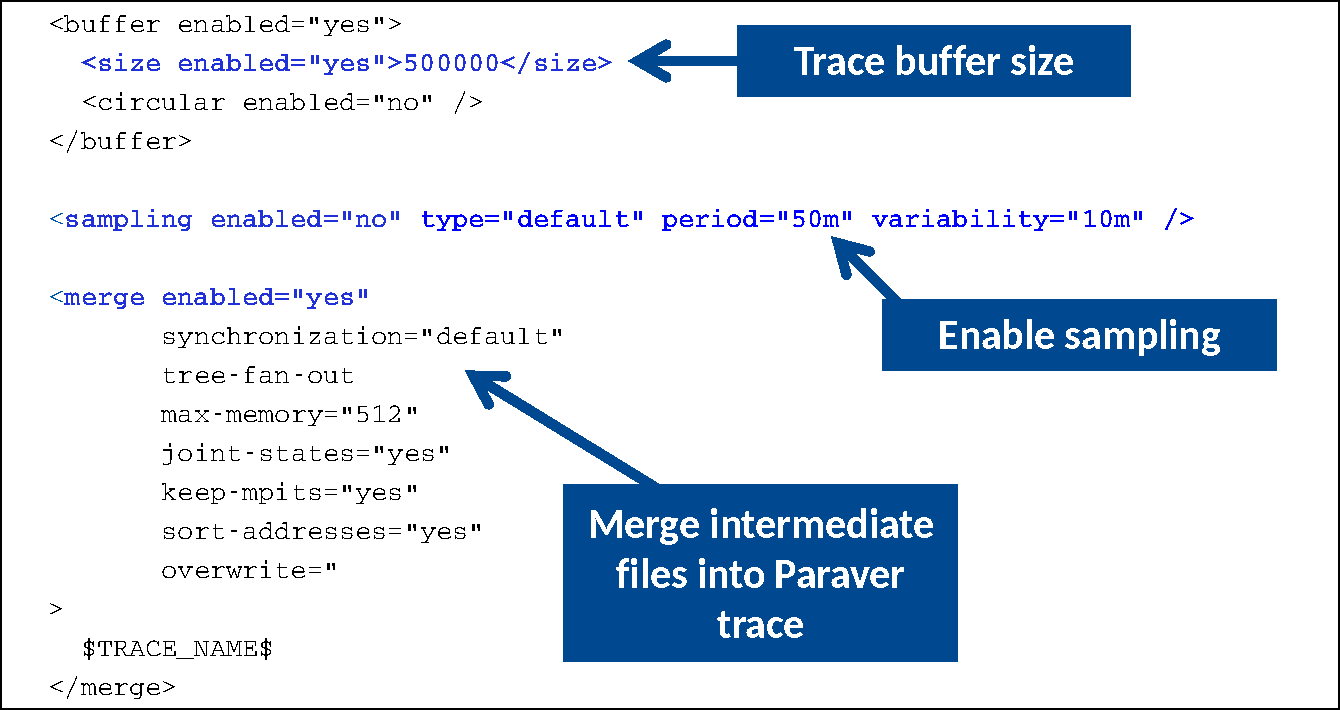
\includegraphics[width=1.1\textwidth]{extraexml3}
  \end{figure}
}

\begin{frame}[fragile]{Extrae: job sumission and trace files}
  \begin{enumerate}
  \item Submit your job!
    \begin{lstlisting}[style=shell,gobble=5]
      sbatch submit_trace.sh   # FT2 submission using SLURM
    \end{lstlisting}
  \item Once finished, the trace is provided in 3 files
    \begin{lstlisting}[style=shell,gobble=5]
      trace_filename.pcv
      trace_filename.prv         # <- the one used by Paraver
      trace_filename.row
    \end{lstlisting}
  \end{enumerate}
\end{frame}



\section{Performance analysis with {\tt paraver}}

\frame{
  \frametitle{Paraver}

  {\bf Paraver}: a flexible performance analysis tool
  \begin{itemize}
  \item Core component in BSC's toolchain
  \item Key design concept:
    \begin{itemize}
    \item provide a qualitative global perception of the application
      behavior by visual inspection
    \item then, focus on the detailed quantitative analysis of the problems
    \end{itemize}

    \pause

  \item Main features: flexible and versatile.\\
    Two main pillars:
    \begin{itemize}
    \item agnostic trace format (no semantics on it)
    \item metrics are not hardwired on the tool but programmed
    \end{itemize}

    \pause

  \item Other features:
    \begin{itemize}
    \item detailed quantitative analysis of program performance
    \item concurrent comparative analysis of several traces
    \item customizable semantics of the visualized information
    \item cooperative work, sharing views of the tracefile
    \item building of derived metrics
    \end{itemize}
  \end{itemize}
}

\frame{
  \frametitle{Paraver: views}

  Two main displays to provide performance information:
  \begin{description}
  \item[Timeline:]
    Behavior of application along time and processes
    \begin{figure}
      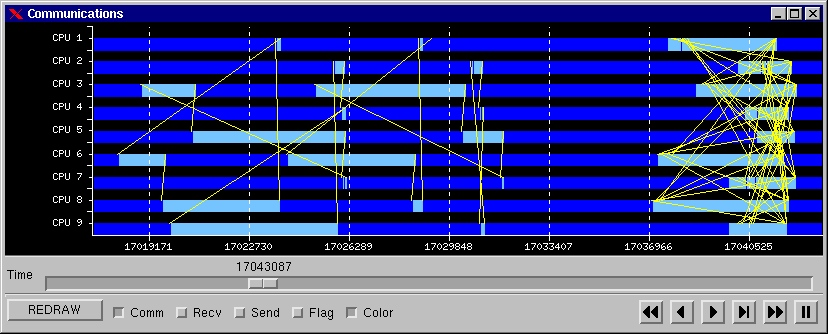
\includegraphics[width=0.7\textwidth]{paravertimeline}
    \end{figure}

    \pause

  \item[Tables:] Numerical analysis of the data
    \begin{itemize}
    \item Profiles, histograms, correlations
    \end{itemize}
    \begin{figure}
      \hspace*{-0.5cm}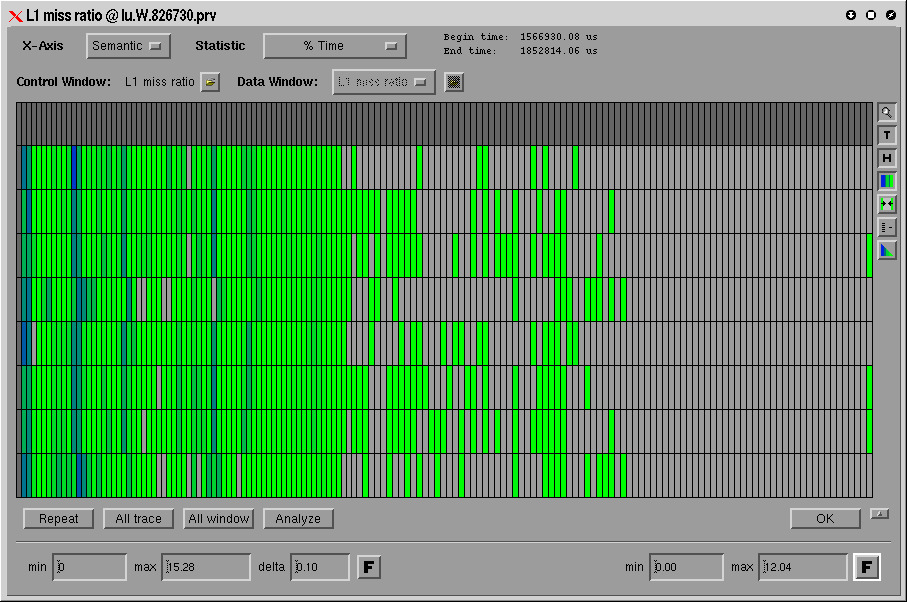
\includegraphics[width=0.4\textwidth]{paraverhistogram}
      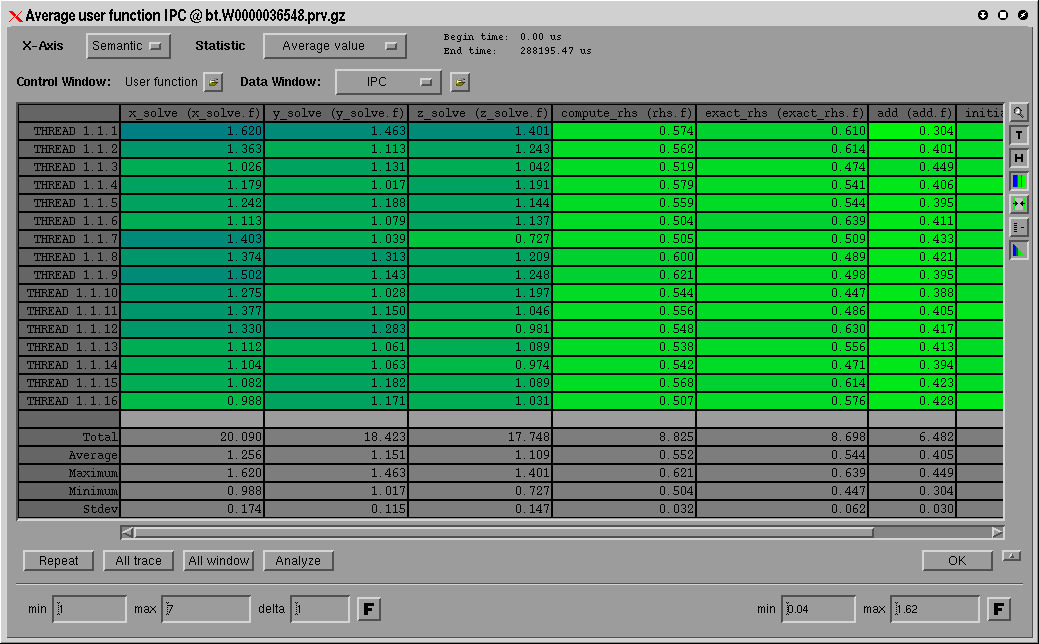
\includegraphics[width=0.43\textwidth]{paraverdata}
    \end{figure}
  \end{description}
}

\frame{
  \frametitle{Paraver, a performance data browser}

  \begin{figure}
    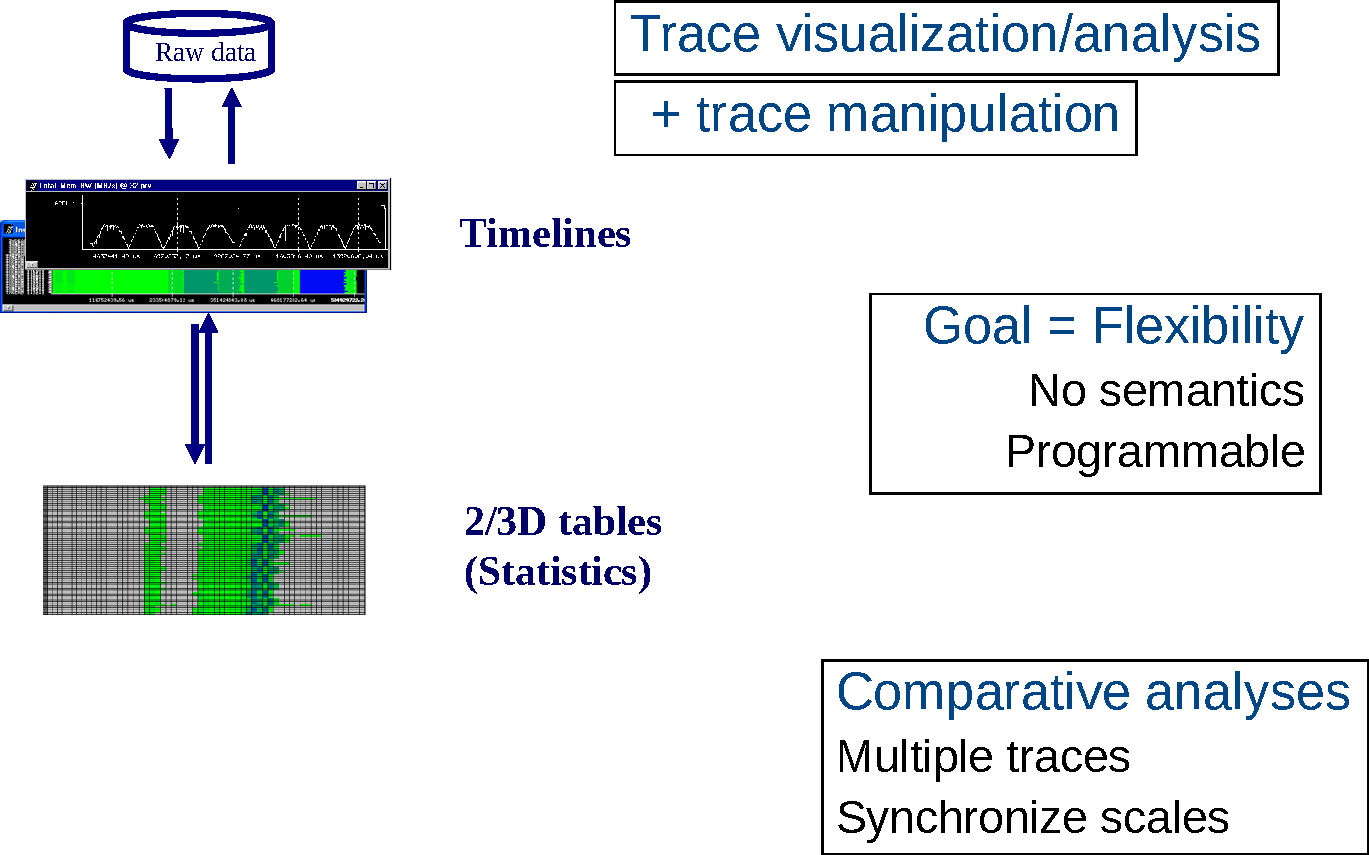
\includegraphics[width=\textwidth]{paraverworkflow}
  \end{figure}
}

\frame{
  \frametitle{Paraver: Profiles, histograms, correlations}

  \begin{figure}
    \hspace*{-0.5cm}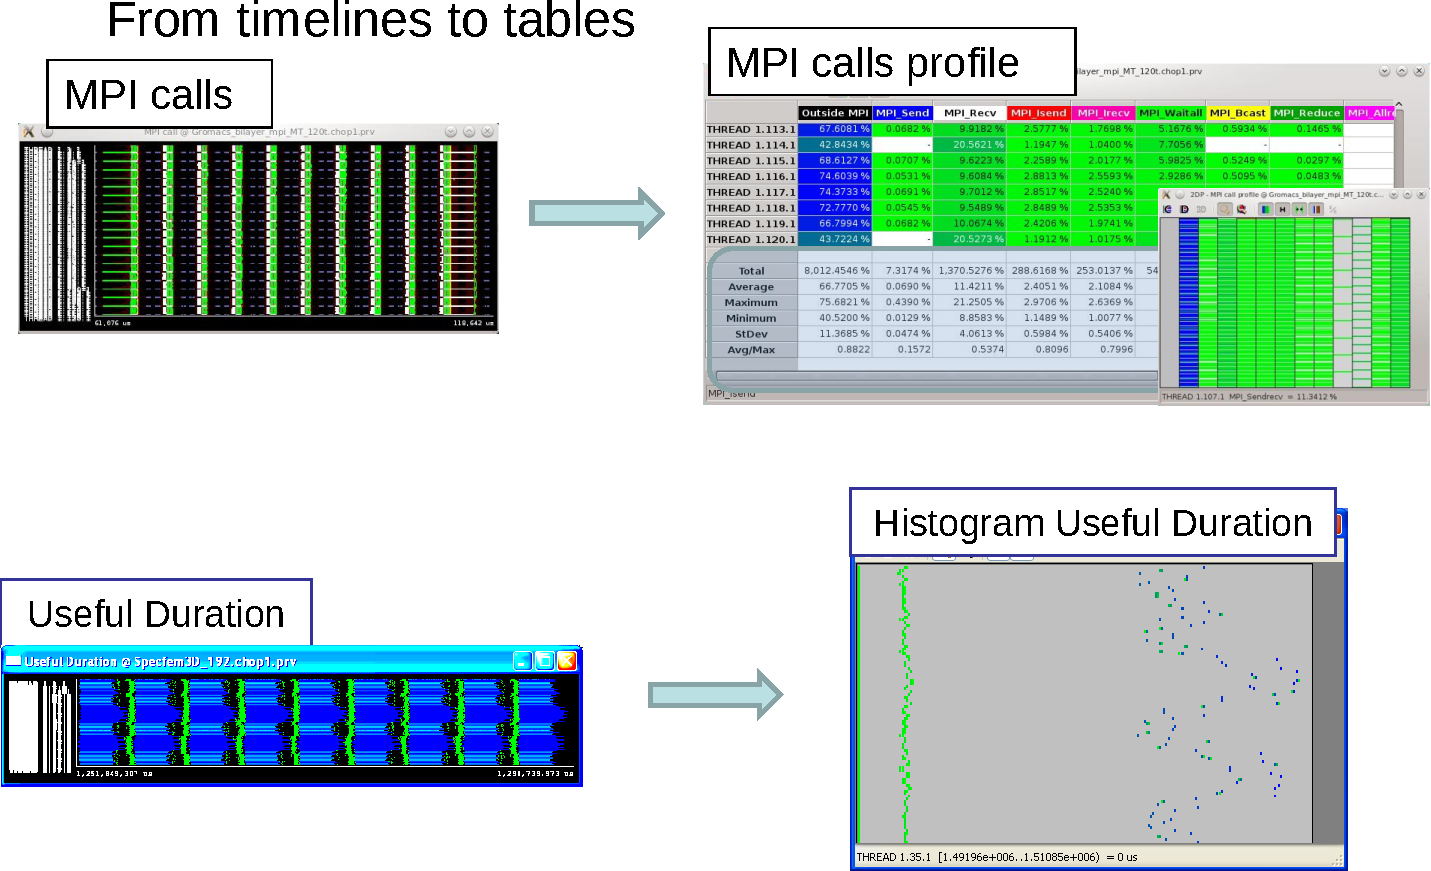
\includegraphics[width=1.1\textwidth]{paravercor}
  \end{figure}
}

\frame{
  \frametitle{Paraver: Analyzing variability through histograms and timelines}

  Key idea in {\tt paraver}: {\bf Gradient}

  \vspace*{-0.3cm}
  \begin{figure}
    \hspace*{-0.5cm}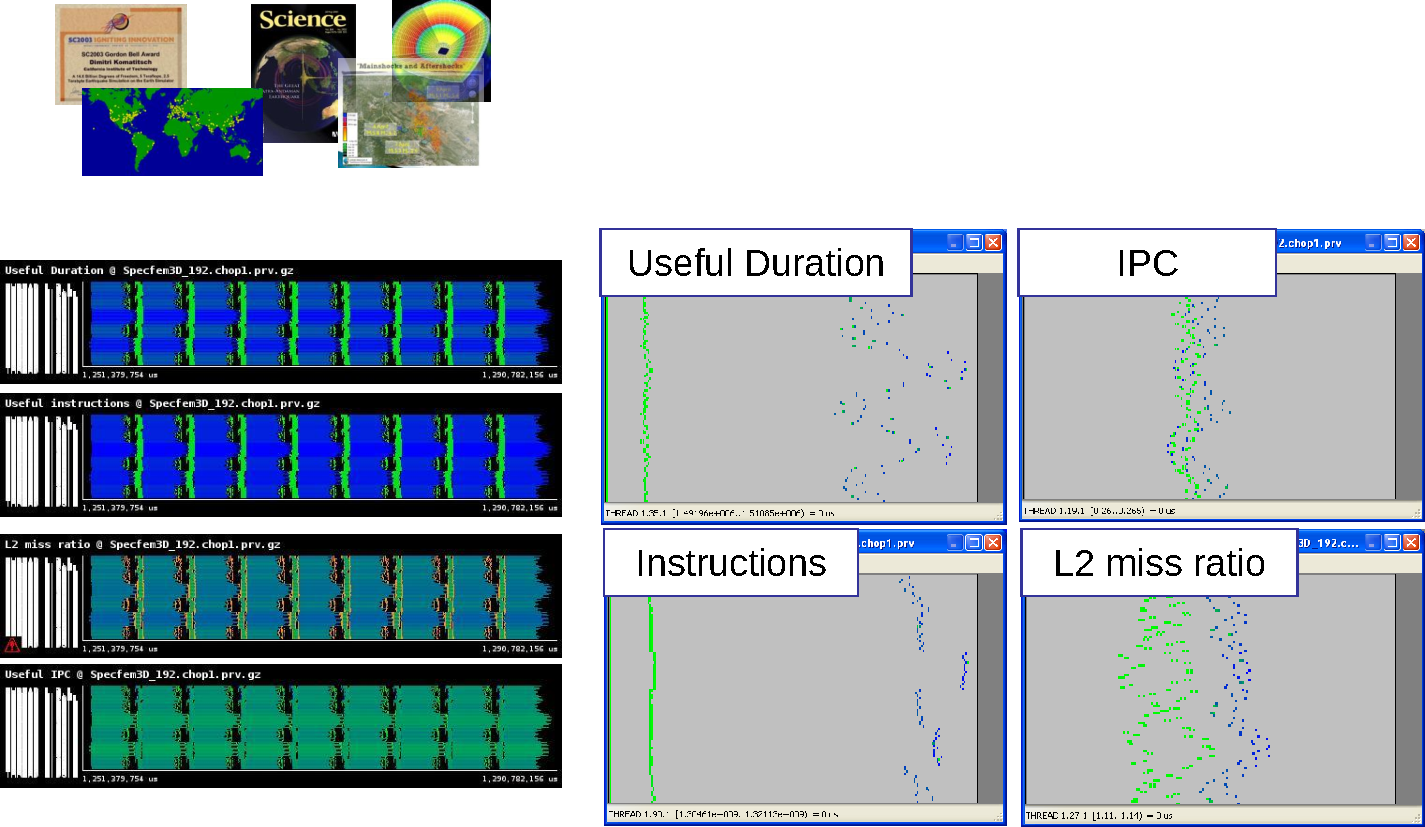
\includegraphics[width=1.1\textwidth]{paraveranal}
  \end{figure}
}

\frame{
  \frametitle{Paraver: Improvement after detecting imbalances}

  After some months of hard work\ldots\footnote{Real experience from a
    BSC experiment}

  \begin{figure}
    \hspace*{-0.8cm}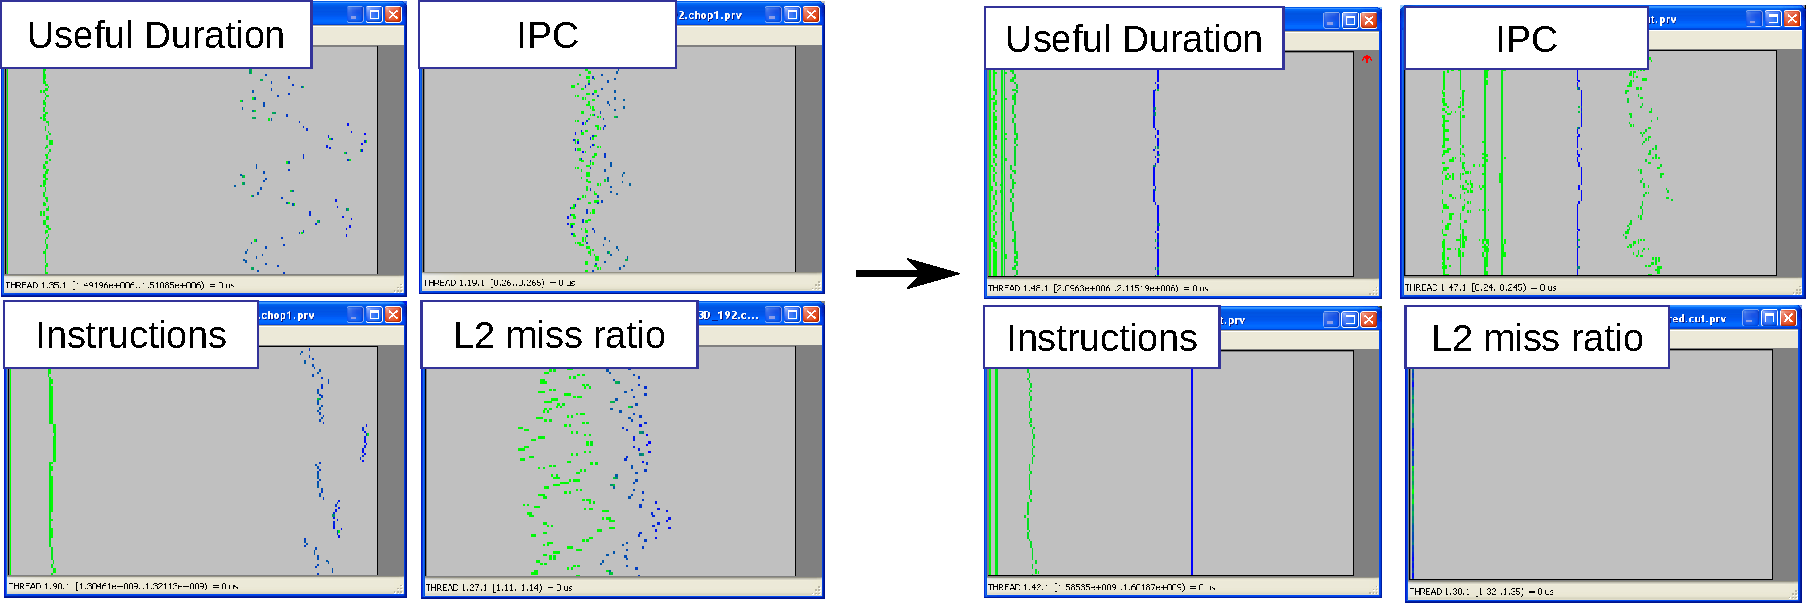
\includegraphics[width=1.15\textwidth]{paraverimprove}
  \end{figure}
}

\frame{
  \frametitle{Paraver: From tables to timelines}

  Where in the timeline do the values in certain table columns appear?
  \vspace*{-0.5cm}
  \begin{itemize}
  \item for example, I want to see the time distribution of a given routine
  \end{itemize}
  \vspace*{-0.2cm}
  \begin{figure}
    \hspace*{-0.8cm}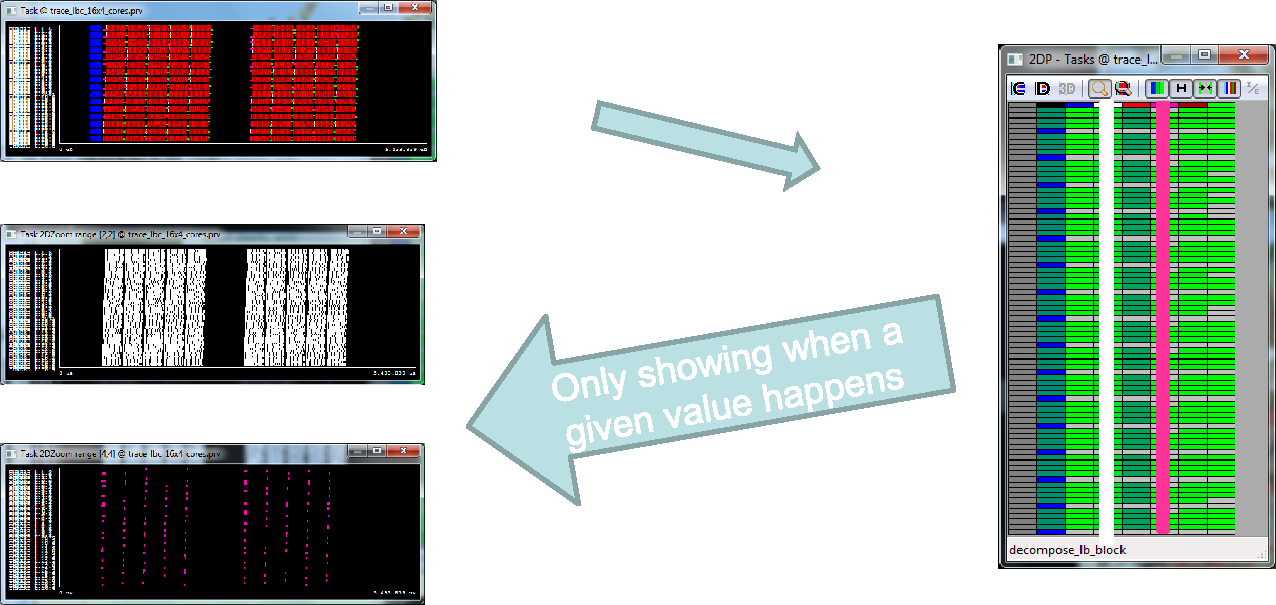
\includegraphics[width=1.15\textwidth]{paravertables}
  \end{figure}
}

\begin{frame}[fragile]{Install {\tt paraver} in your computer}
  \begin{itemize}
  \item Download {\tt paraver} from the official site:\\
    \hfil \url{https://tools.bsc.es/downloads}
  \item Download the tutorials and uncompress them into the {\tt
      paraver} directory:\\
    \hfil \url{https://tools.bsc.es/paraver-tutorials}
  \item Launch paraver. For example: (use your installation path)
    \begin{lstlisting}[style=shell,gobble=3]
      /opt/wxparaver-4.7.2-Linux_x86_64/bin/wxparaver
    \end{lstlisting}
  \item Check the tutorials: {\small (also available in pdf and html)}\\
    \hfil Help$\rightarrow$Tutorials
  \end{itemize}
\end{frame}


%\section{Parametric analysis of behaviour with {\tt dimemas}}

%\begin{frame}
%\end{frame}

\section{Visualization and optimization of shared memory parallelized codes}


\begin{frame}{Factors that influence the obtainable performance of a parallel implementation}
\begin{itemize}
    \item Amdahl's Law: It quantifies the obtainable acceleration considering the fraction of the execution time affected by the parallelization and the speedup applied to that part
    \item Sequential algorithm vs Parallel algorithm: The algorithm use to solve a problem might be different for the sequential and the parallel implementations. The parallel implementation sometimes uses a more complex (but more parallelizable) algorithm
    \item Waits, Locks \& Synchronizations imposed by the use of a parallel library
\end{itemize}    
\end{frame}


\begin{frame}{Shared-memory parallelized codes}
\begin{itemize}
    \item These codes use all the cores available within a node of a supercomputer/cluster
    \item In order to do this, several threads/tasks are executed concurrently
    \item It can ben combined with vectorization that happens within each core
    \item There are different libraries to exploit this kind of parallelism
        \begin{itemize}
            \item OpenMP (The most common one) \uncover<2>{\textcolor{red}{We will focus on this study case}}
            \item Intel Threading Building Blocks
            \item Intel Task Parallel Library
            \item Message Passing Interface (MPI): although this library is mainly used for distributed-memory environments
            \item OpenCL: although this library is mainly used for GPGPU
        \end{itemize}
\end{itemize}
\end{frame}

\subsection{Small intro to OpenMP}

\begin{frame}{Small intro to OpenMP}
\emph{OpenMP}\footnote{\url{https://computing.llnl.gov/tutorials/openMP/}}  is a parallel-programming API for shared-memory environments that can be used in virtually any desktop operative system (Linux, MacOS, Windows,\ldots)

Languages supported:
\begin{itemize}
    \item C/C++
    \item Fortran
\end{itemize}

Main OpenMP components:
\begin{itemize}
    \item Compiler directives (a.k.a. pragmas)
    \item Library routines
    \item Environment variables
\end{itemize}

\end{frame}

\begin{frame}[fragile]{Small intro to OpenMP: Compiler directives}
OpenMP compiler directives\footnote{\url{https://computing.llnl.gov/tutorials/openMP/\#Directives}}  appear on your code and they are ignored although you indicate otherwise to the compiler
\begin{description}
\item[In GCC:] gcc -fopenmp
\item[In ICC:] icc -openmp
\end{description}
%https://computing.llnl.gov/tutorials/openMP/
%and in general https://hpc.llnl.gov/training/tutorials

General form of a compiler directive

\begin{verbatim}
#pragma sentinel directive-name [clause, ...]
\end{verbatim}

OpenMP example:

\begin{verbatim}
#omp parallel default(shared) private(a,b)
\end{verbatim}

\end{frame}

\begin{frame}[fragile]{Small intro to OpenMP: Run-time library routines}
The OpenMP API includes an ever-growing number of run-time library routines\footnote{\url{https://computing.llnl.gov/tutorials/openMP/\#RunTimeLibrary}} .

These routines are used for a variety of purposes:

\begin{itemize}
    \tiny
    \item Setting and querying the number of threads
    \item Querying a thread's unique identifier (thread ID), a thread's ancestor's identifier, the thread team size
    \item Setting and querying the dynamic threads feature
    \item Querying if in a parallel region, and at what level
    \item Setting and querying nested parallelism
    \item Setting, initializing and terminating locks and nested locks
    \item Querying wall clock time and resolution
\end{itemize}

If you want to use them you have to include the headers

\begin{verbatim}
    #include <omp.h>
\end{verbatim}

An example

\begin{verbatim}
    int omp_get_num_threads(void);
\end{verbatim}

\end{frame}

\begin{frame}[fragile]{Small intro to OpenMP: Environment variables}
OpenMP provides several environment variables\footnote{\url{https://computing.llnl.gov/tutorials/openMP/\#EnvironmentVariables}} for controlling the execution of parallel code at run-time.

These environment variables can be used to control such things as:
\begin{itemize}
    \tiny
    \item Setting the number of threads
    \item Specifying how loop iterations are divided
    \item Binding threads to processors
    \item Enabling/disabling nested parallelism; setting the maximum levels of nested parallelism
    \item Enabling/disabling dynamic threads
    \item Setting thread stack size
    \item Setting thread wait policy
\end{itemize}

An example

\begin{verbatim}
export OMP_NUM_THREADS=8
\end{verbatim}
    
\end{frame}

\begin{frame}[fragile]{Small intro to OpenMP: Parallel region construct}

A parallel region is a block of code that will be executed by multiple threads.

Syntax:

\begin{verbatim}
    #pragma omp parallel [clause ...] newline
    
    structured_block
\end{verbatim}
Possible clauses\footnote{\url{https://computing.llnl.gov/tutorials/openMP/\#Clauses}}:
    \begin{description}
    \footnotesize
    \item[private (list)] It declares variables in its list to be private to each thread
    \item[shared (list)] It declares variables in its list to be shared among all the thread in the team
    \item[default (shared|none)]It allows the user to specify a default scope for all variables in the lexical extent of any parallel region.
    \item[] \ldots
    \end{description}

\end{frame}

\begin{frame}[fragile]{Small intro to OpenMP: Work-sharing constructs}

The DO / for directive specifies that the iterations of the loop immediately following it must be executed in parallel by the team.

Syntax:

\begin{verbatim}
    #pragma omp for [clause ...]  newline    
    
    for_loop
\end{verbatim}

The SINGLE directive specifies that the enclosed code is to be executed by only one thread in the team.

Syntax:

\begin{verbatim}
    #pragma omp single [clause ...]  newline 
    
    structured_block
\end{verbatim}

\end{frame}

\begin{frame}[fragile]{Small intro to OpenMP: Task construct}
The task construct\footnote{\url{https://computing.llnl.gov/tutorials/openMP/\#Task}}  defines an explicit task, which may be executed by the encountering thread, or deferred for execution by any other thread in the team.

\begin{verbatim}
    #pragma omp task [clause ...]  newline 

    structured_block
\end{verbatim}
\end{frame}

\begin{frame}[fragile]{Small intro to OpenMP: Depend clause}
The depend clause\footnote{\url{http://www.nersc.gov/users/software/programming-models/openmp/openmp-tasking/}} (available since OpenMP 4.0) takes a type followed by a variable or list of variables.

\begin{verbatim}
#pragma omp task depend(in: x) depend( out: y) 
                 depend(inout: z)    
\end{verbatim}

The (address of) variables passed to the depend clause are used to correctly order the tasks. These constraints are determined by the type of dependency specified:

\begin{itemize}
\footnotesize
\item IN dependencies will make a task dependent on the last task that used the same variable as an out (or inout) dependency. 
\item OUT dependencies will make a task dependent on the last task that used the same variable as an in, out (or inout) dependency.
\item INOUT dependencues are the same as an out dependency, they are only used for readability.
\end{itemize}
\end{frame}


\subsection{Solving with Extrae and Paraver common issues in shared-memory parallelized programs}

\begin{frame}{Most useful configurations of Paraver}
\centering
OpenMP->Analysis->omp\_profile.cfg (Table)

\begin{columns}
\begin{column}{0.5\textwidth}
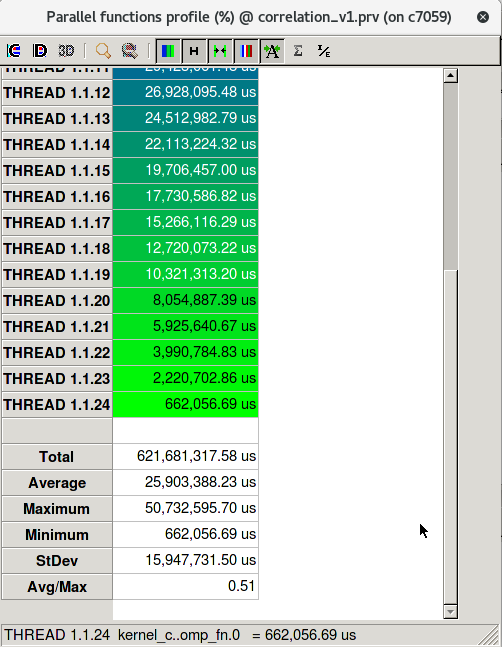
\includegraphics[width=\textwidth]{figs/omp_profile_table.png}
\end{column}
\begin{column}{0.5\textwidth}
  \begin{itemize}
      \item One column per parallel region
      \item One row per thread
      \item Contains duration of each thread
      \item Load imbalance is detected by Avg/Max statistic
  \end{itemize}
\end{column}
\end{columns}
\end{frame}

\begin{frame}{Most useful configurations of Paraver}
\centering
OpenMP->Analysis->omp\_profile.cfg (Timeline)

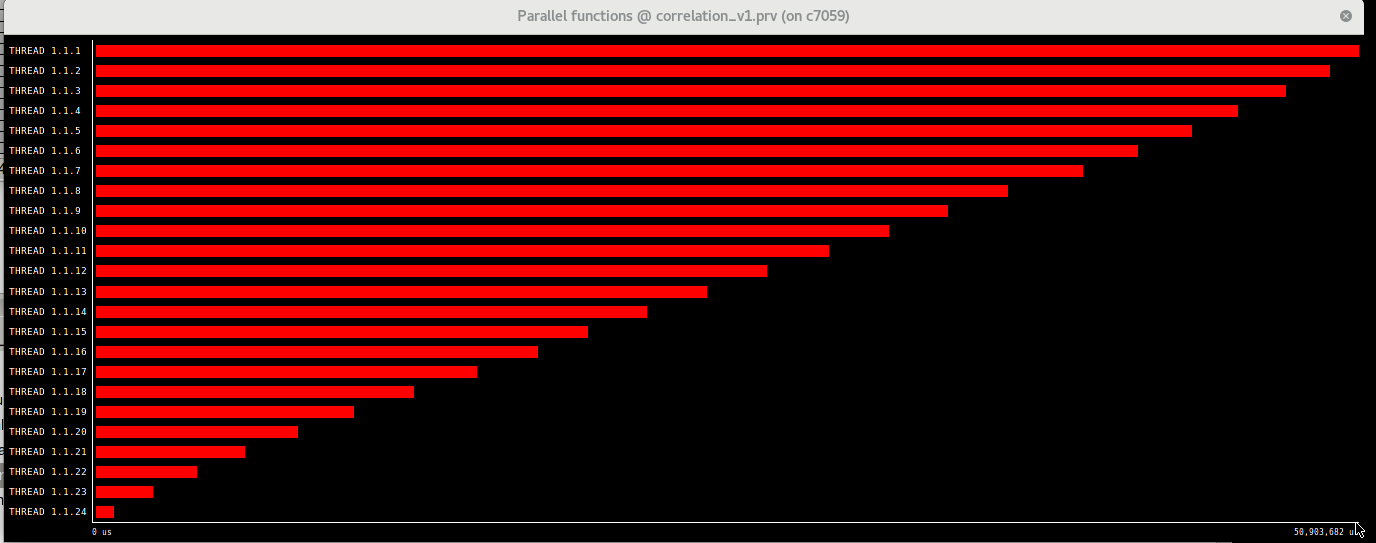
\includegraphics[width=0.8\textwidth]{figs/omp_profile_timeline.png}

It shows the execution of thread through time. 
\end{frame}

\begin{frame}{Common issues in shared-memory parallelized programs}
\begin{description}
\item[Issue \#1] Locks and waits due to suboptimal usage of the parallel library
\item[Issue \#2] Load imbalance
\item[Issue \#3] False sharing
\item[Issue \#4] Inadequate tasks exploitation
\item[Issue \#5] Poor locality
\end{description}
\end{frame}

\begin{frame}{Issue \#1: Locks and waits due to suboptimal usage of the parallel library}
Examples of this in OpenMP are:
\begin{itemize}
    \item Avoid the critical region construct
    \item Avoid large critical regions
    \item Maximize parallel regions
    \item Avoid parallel regions in inner loops
\end{itemize}
\end{frame}

\begin{frame}[fragile]{An example of Issue \#1 in Paraver (code01)}
The difference between these two version of the same code is really subtle
\begin{columns}
\begin{column}{0.57\textwidth}
\begin{lstlisting}[style=shell,basicstyle=\scriptsize\ttfamily,gobble=3,caption={Several parallel regions}]
     #pragma omp parallel for private (i)
    for (j = 0; j < _PB_M; j++)
    (...)
    #pragma omp parallel for private (i)
    for (j = 0; j < _PB_M; j++)
    (...)
    
    #pragma omp parallel for private (j)
    for (i = 0; i < _PB_N; i++)
    (...)
    #pragma omp parallel for private (j2, i)
    for (j1 = 0; j1 < _PB_M-1; j1++)
    (...)
  \end{lstlisting}
  \end{column}
\begin{column}{0.43\textwidth}
  \begin{lstlisting}[style=shell,gobble=3,basicstyle=\scriptsize\ttfamily,caption={One parallel region}]
   #pragma omp parallel
  {
    #pragma omp for private (i)
    for (j = 0; j < _PB_M; j++)
    (...)
    #pragma omp for private (i)
    for (j = 0; j < _PB_M; j++)
    (...)
    #pragma omp for private (j)
    for (i = 0; i < _PB_N; i++)
    (...)
    #pragma omp for private (j2, i)
    for (j1 = 0; j1 < _PB_M-1; j1++)
    (...)
  }
  \end{lstlisting}
  \end{column}
  \end{columns}
\end{frame}

\begin{frame}{An example of Issue \#1 in Paraver (code01)}
The different in the visualization when zooming in the first three loops are noticeable
\centering
\begin{columns}
\begin{column}{0.5\textwidth}
\\\underline{With several parallel regions}
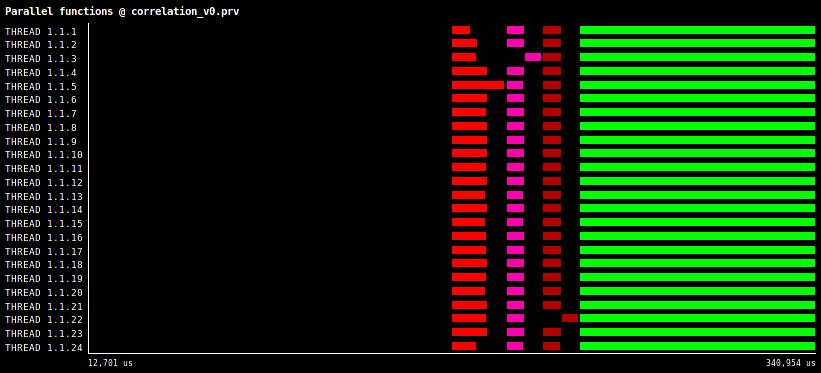
\includegraphics[width=0.99\textwidth]{figs/Parallel_functions@correlation_v0.png}
 \end{column}
 \begin{column}{0.5\textwidth}
 \\\underline{With one parallel region}
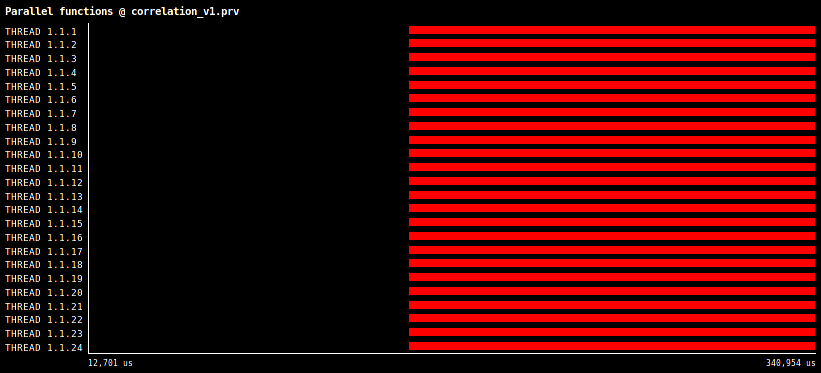
\includegraphics[width=0.99\textwidth]{figs/Parallel_functions@correlation_v1.png}
 \end{column}
\end{columns}
\end{frame}

\begin{frame}{An example of Issue \#1 in Paraver (code01)}
Do it yourself
\begin{itemize}
    \item Connect to FT2 with X export: {\tt ssh -X youruser@ft6.cesga.es}
    \item Clone the repository: {\tt git clone https://github.com/diegoandradecanosa/extraeCoursecodes}
    \item Enter in directory code01: {\tt cd extraeCoursecodes/code01}
    \item Generate the traces (they have already been generated by me): {\tt ./generatetraces.sh}
    \item Load the paraver module:  {\tt module load paraver}
    \item Load the first trace: {\tt wxparaver correlation\_v0.prv}
    \item Visualize using configuration OpenMP/analysis/omp\_profile.cfg -> Open Control Window -> Zoom in the first part of the trace
    \item Do the same for the other trace correlation\_v1.prv
\end{itemize}
\end{frame}

\begin{frame}{Issue \#2: Load imbalance}
It is a big issue in irregular computations, such as:
\begin{itemize}
    \item Triangular loops
    \item Parallel traversing of linked lists
    \item Also, when the body of the parallel loop has conditional statements
\end{itemize}
\end{frame}

\begin{frame}[fragile]{An example of Issue \#2 in Paraver (code02)}
These two codes distribute the same workload using different policies
\begin{columns}
\begin{column}{0.5\textwidth}
\begin{lstlisting}[style=shell,basicstyle=\scriptsize\ttfamily,gobble=3,caption={Default scheduling}]
    #pragma omp for private (j, k)
    for (i = 1; i < _PB_NI; i++)
      for (j = 0; j < _PB_NI; j++)
        for (k = 0; k < i; k++)
  \end{lstlisting}
  \end{column}
\begin{column}{0.5\textwidth}
  \begin{lstlisting}[style=shell,gobble=3,basicstyle=\scriptsize\ttfamily,caption={Load-balance-aware scheduling}]
    #pragma omp for private (j, k) 
            schedule(static,8)
    for (i = 1; i < _PB_NI; i++)
      for (j = 0; j < _PB_NI; j++)
	    for (k = 0; k < i; k++)
  \end{lstlisting}
  \end{column}
  \end{columns}
\end{frame}

\begin{frame}{An example of Issue \#2 in Paraver (code02)}
A visualization of the corresponding traces with Paraver reveals that the work in the second version is more balanced
\centering
\begin{columns}
\begin{column}{0.5\textwidth}
\\\underline{Imbalance}
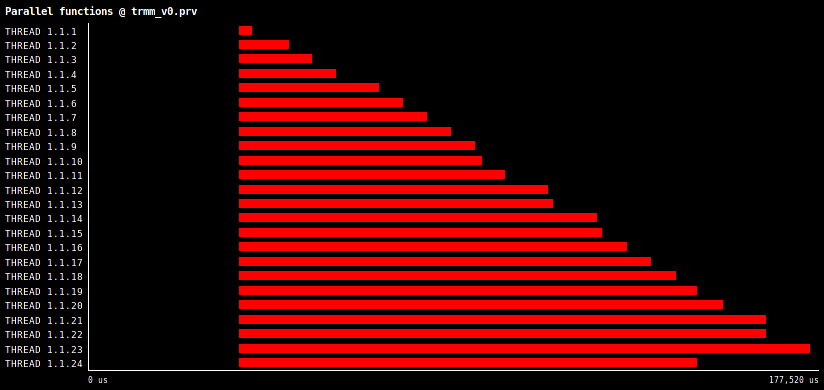
\includegraphics[width=0.99\textwidth]{figs/Parallel_functions@trmm_v0.png}
 \end{column}
 \begin{column}{0.5\textwidth}
 \\\underline{More balanced}
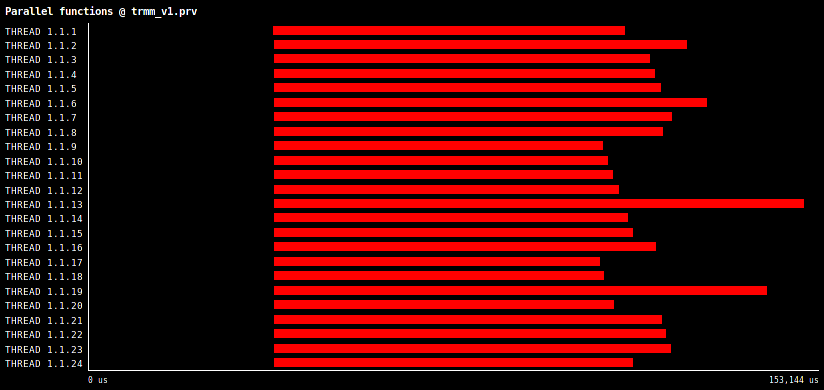
\includegraphics[width=0.99\textwidth]{figs/Parallel_functions@trmm_v1.png}
 \end{column}
\end{columns}
\end{frame}


\begin{frame}{An example of Issue \#2 in Paraver (code02)}
Do it yourself
\begin{itemize}
    \item Connect to FT2 with X export: {\tt ssh -X youruser@ft6.cesga.es}
    \item Clone the repository: {\tt git clone https://github.com/diegoandradecanosa/extraeCoursecodes}
    \item Enter in directory code02: {\tt cd extraeCoursecodes/code02}
    \item Generate the traces (they have already been generated by me): {\tt ./generatetraces.sh}
    \item Load the paraver module:  {\tt module load paraver}
    \item Load the first trace: {\tt wxparaver trmm\_v0.prv}
    \item Visualize using configuration OpenMP/analysis/omp\_profile.cfg -> Open Control Window -> Zoom in the first part of the trace
    \item Do the same for the other trace trmm\_v1.prv
\end{itemize}
\end{frame}


\begin{frame}{Issue \#3: False sharing}
False sharing is a situation where two different threads are accessing different  parts of the same cache line
\begin{itemize}
    \footnotesize
    \item It is performance issue if both threads are modifying that data
    \item The problem is that the cache coherency protocol cannot identify that they are accessing disjunct parts of the same cache line, thus, the line is invalidated in one of the cores
    \item In OpenMP it usually happens when we use a static block-cyclic distribution with a small chunk size
    \item It usually leads to poor scaling
\end{itemize}
\centering
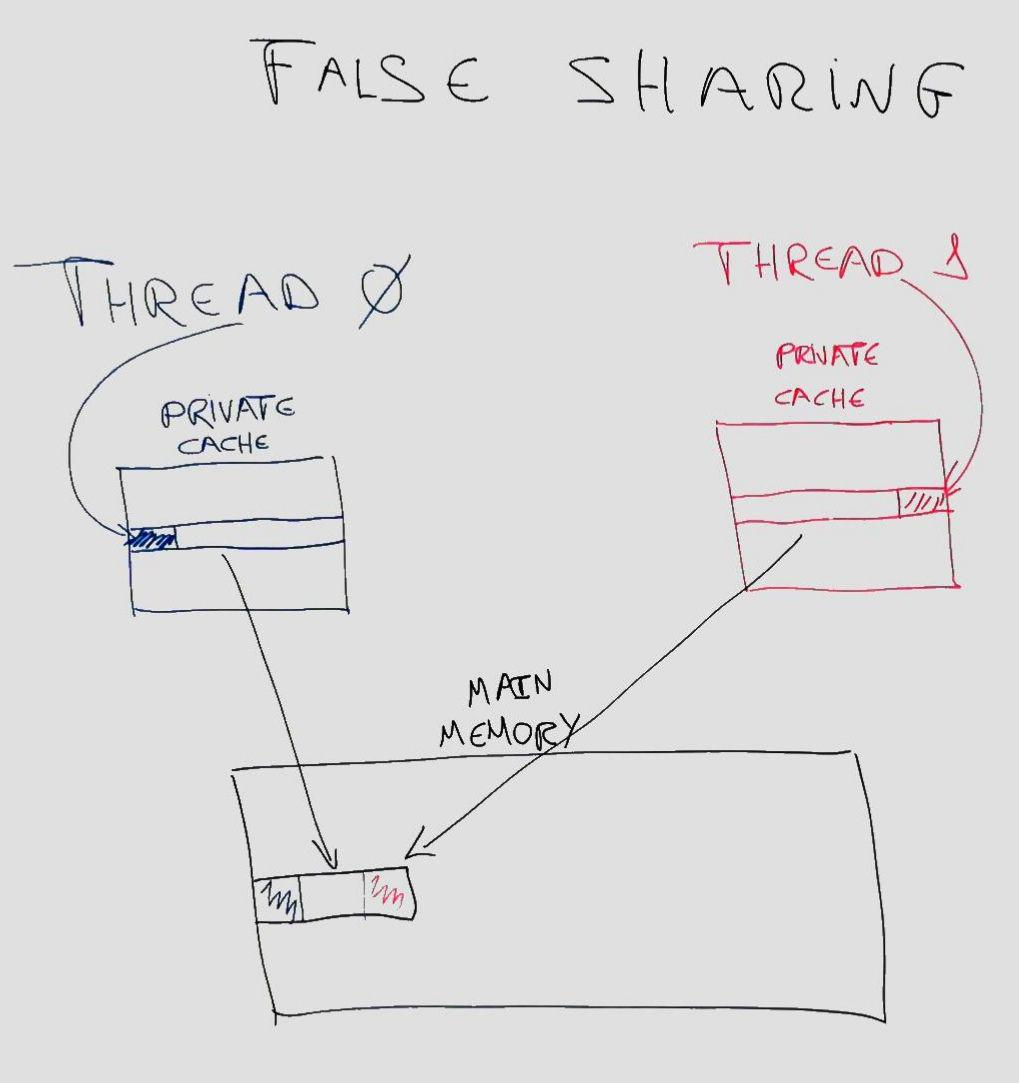
\includegraphics[width=0.4\textwidth]{figs/myfalsesharing.jpg}
\end{frame}

\begin{frame}[fragile]{An example of Issue \#3 in Paraver (code03)}
The first version of the Biconjugate Gradient (BICG) method has fal sharing, due to the work distribution policy, the second one don't
\begin{columns}
\begin{column}{0.5\textwidth}
\begin{lstlisting}[style=shell,basicstyle=\scriptsize\ttfamily,gobble=3,caption={With False Sharing (v0)}]
    #pragma omp for schedule(static,1)
    for (i = 0; i < _PB_NY; i++)
      s[i] = 0;
    #pragma omp for private (j) 
    schedule(static,1)
    for (i = 0; i < _PB_NX; i++)
      {
        q[i] = 0;
        for (j = 0; j < _PB_NY; j++)
          {
            s[j] = s[j] + r[i] * A[i][j];
            q[i] = q[i] + A[i][j] * p[j];
          }
      }

  \end{lstlisting}
  \end{column}
\begin{column}{0.5\textwidth}
  \begin{lstlisting}[style=shell,gobble=3,basicstyle=\scriptsize\ttfamily,caption={Without False Sharing (v1)}]
    #pragma omp for
    for (i = 0; i < _PB_NY; i++)
      s[i] = 0;
    #pragma omp for private (j)
    for (i = 0; i < _PB_NX; i++)
      {
        q[i] = 0;
        for (j = 0; j < _PB_NY; j++)
          {
            s[j] = s[j] + r[i] * A[i][j];
            q[i] = q[i] + A[i][j] * p[j];
          }
      }

  \end{lstlisting}
  \end{column}
  \end{columns}
\end{frame}

\begin{frame}{Issue \#3: False sharing}
\centering
L2 Miss rate of v0 (false sharing)\\
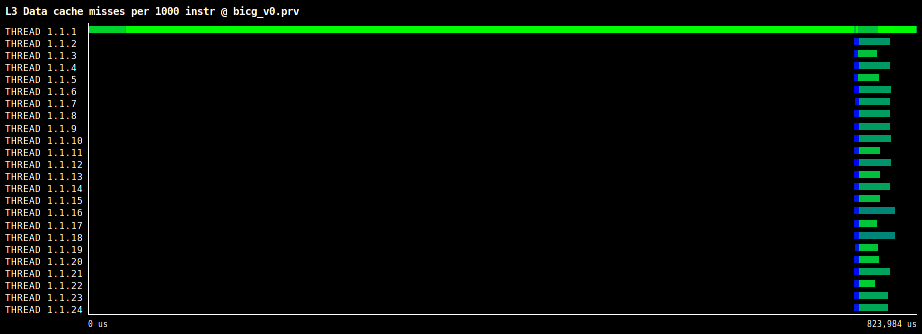
\includegraphics[width=0.8\textwidth]{figs/L3_Data_cache_misses_per_1000_instr@bicg_v0.png}\\
L2 Miss rate of v1 (no false sharing)\\
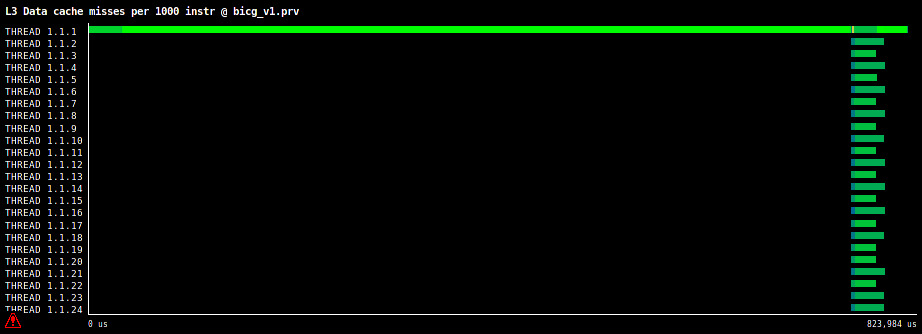
\includegraphics[width=0.8\textwidth]{figs/L3_Data_cache_misses_per_1000_instr@bicg_v1.png}\\
\end{frame}

\begin{frame}{An example of Issue \#3 in Paraver (code03)}
Do it yourself
\begin{itemize}
    \item Connect to FT2 with X export: {\tt ssh -X youruser@ft6.cesga.es}
    \item Clone the repository: {\tt git clone https://github.com/diegoandradecanosa/extraeCoursecodes}
    \item Enter in directory code03: {\tt cd extraeCoursecodes/code03}
    \item Generate the traces (they have already been generated by me): {\tt ./generatetraces.sh}
    \item Load the paraver module:  {\tt module load paraver}
    \item Load the first trace: {\tt wxparaver bicg\_v0.prv}
    \item Visualize using configuration extraeCoursecodes/common/cfgs/L2MissRate.cfg 
    \item Do the same for the other trace bicg\_v1.prv
\end{itemize}
\end{frame}

\begin{frame}{Issue \#4: Inadequate tasks exploitation}
Tasks and task dependencies are a powerful parallelization mechanism, but the performance is highly dependent of the design of the parallel implementation

And there are many possible alternate implementations
%http://www.nersc.gov/users/software/programming-models/openmp/openmp-tasking/openmp-tasking-example-jacobi/
\end{frame}

\begin{frame}[fragile]{An example of Issue \#4 in Paraver (code04)}
This example is based on a Jacobi 2D Stencil computation. There are three versions of the paralle implementation of this code. 
\begin{lstlisting}[style=shell,basicstyle=\scriptsize\ttfamily,gobble=3,caption={Parallelized with for pragmas (v0)}]
     for (t = 0; t < _PB_TSTEPS; t++)
      {
        #pragma omp for schedule(static) 
        for (i = 1; i < _PB_N - 1; i++)
          for (j = 1; j < _PB_N - 1; j++)
            B[i][j] = 0.2 * (A[i][j] 
            + A[i][j-1] + A[i][1+j] 
            + A[1+i][j] + A[i-1][j]);
        #pragma omp for schedule(static) 
        for (i = 1; i < _PB_N-1; i++)
          for (j = 1; j < _PB_N-1; j++)
            A[i][j] = B[i][j];
      }
    }
  \end{lstlisting}
\end{frame}

\begin{frame}[fragile]{An example of Issue \#4 in Paraver (code04)}
This example is based on a Jacobi 2D Stencil computation. There are three versions of the paralle implementation of this code. 
  \begin{lstlisting}[style=shell,gobble=3,basicstyle=\scriptsize\ttfamily,caption={Parallelized with tasks (v1)}]
      for (t = 0; t < _PB_TSTEPS; t++)
      {
        for (i = 1; i < _PB_N - 1; i++)
        #pragma omp depend(in: A[j], A[j+_PB_N], src[j-_PB_N]) 
        depend(out: B[j])   
          for (j = 1; j < _PB_N - 1; j++)
            B[i][j] = 0.2 * (A[i][j] 
            + A[i][j-1] + A[i][1+j] 
            + A[1+i][j] + A[i-1][j]);
        #pragma omp for schedule(static) 
        for (i = 1; i < _PB_N-1; i++)
          for (j = 1; j < _PB_N-1; j++)
            A[i][j] = B[i][j];
      }
    }
  \end{lstlisting}
\end{frame}

\begin{frame}{An example of Issue \#4 in Paraver (code04)}
\centering
OMP profile of v0\\
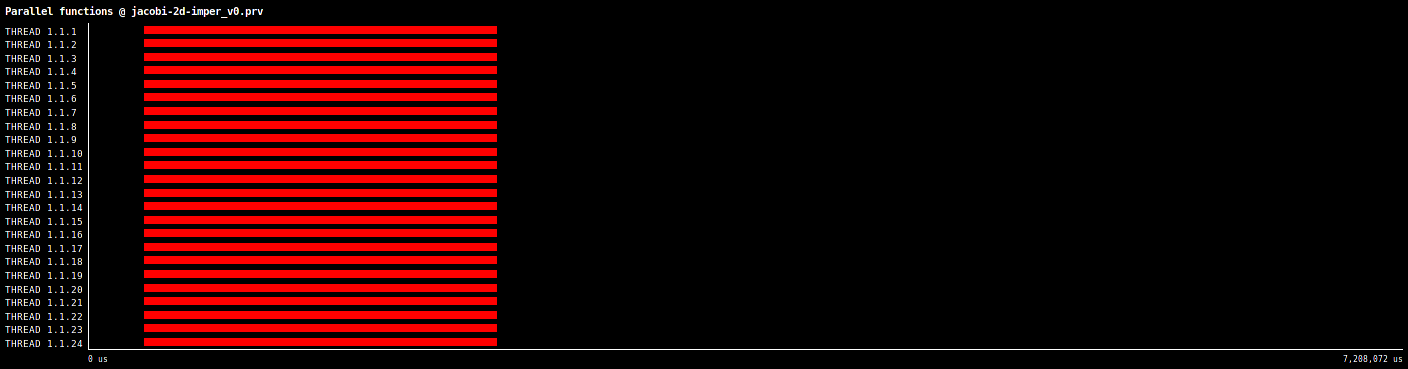
\includegraphics[width=0.8\textwidth]{figs/Parallel_functions@jacobi-2d-imper_v0.png}\\
OMP profile of v1\\
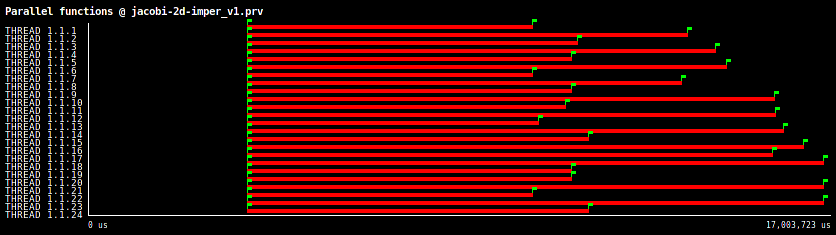
\includegraphics[width=0.8\textwidth]{figs/Parallel_functions@jacobi-2d-imper_v1.png}\\
OMP profile of v2\\
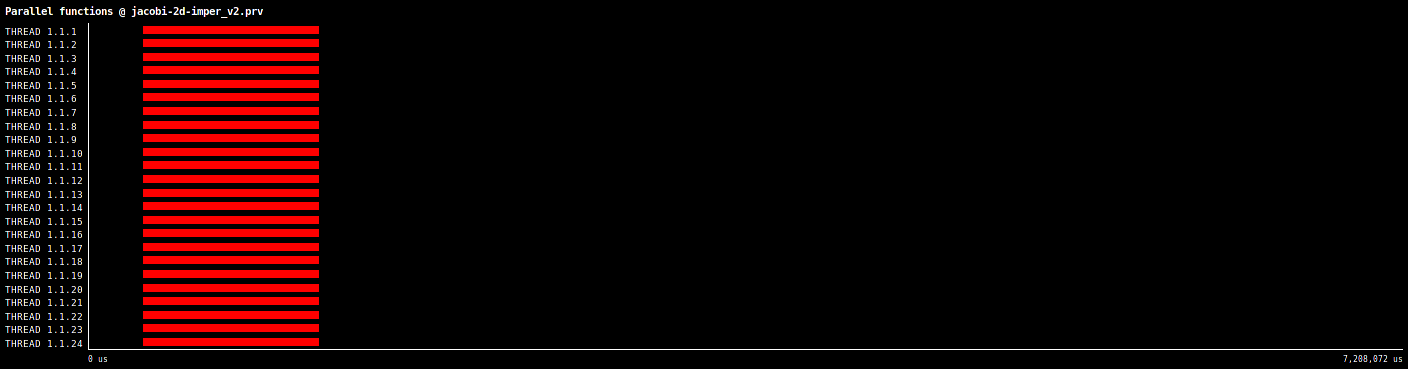
\includegraphics[width=0.8\textwidth]{figs/Parallel_functions@jacobi-2d-imper_v2.png}\\
\end{frame}
\begin{frame}[fragile]{An example of Issue \#4 in Paraver (code04)}
This example is based on a Jacobi 2D Stencil computation. There are three versions of the paralle implementation of this code. 
\begin{lstlisting}[style=shell,basicstyle=\scriptsize\ttfamily,gobble=3,caption={Parallelized with tasks (v2)}]
      for (t = 0; t < _PB_TSTEPS; t++)
      {
        for (i = 1; i < _PB_N - 1; i++)
        #pragma omp depend(in:B[jj],B[jj+_PB_N]
        , B[jj+_PB_N]) depend(out: A[jj])
         for(j=i;j<((j+chunk_size) && (j< _PB_N-1));j=j+chunk_size)
          for (jj = (j*_PB_N)+1; jj < ((j*_PB_N)+_PB_N - 1); jj++)
            B[i][jj] = 0.2 * (A[i][jj] 
            + A[i][jj-1] + A[i][1+jj] 
            + A[1+i][jj] + A[i-1][jj]);
        #pragma omp for schedule(static) 
        for (i = 1; i < _PB_N-1; i++)
          for (j = 1; j < _PB_N-1; j++)
            A[i][j] = B[i][j];
      }
    }

  \end{lstlisting}

\end{frame}


\begin{frame}{An example of Issue \#4 in Paraver (code04)}
Do it yourself
\begin{itemize}
    \item Connect to FT2 with X export: {\tt ssh -X youruser@ft6.cesga.es}
    \item Clone the repository: {\tt git clone https://github.com/diegoandradecanosa/extraeCoursecodes}
    \item Enter in directory code04: {\tt cd extraeCoursecodes/code04}
    \item Generate the traces (they have already been generated by me): {\tt ./generatetraces.sh}
    \item Load the paraver module:  {\tt module load paraver}
    \item Load the first trace: {\tt wxparaver jacobi-2d-imper\_v0.prv}
    \item Visualize using configuration OpenMP/analysis/omp\_profile.cfg -> Open Control Window -> Zoom in the first part of the trace
    \item Do the same for the other two traces jacobi-2d-imper\_v0.prv jacobi-2d-imper\_v1.prv jacobi-2d-imper\_v2.prv
\end{itemize}
\end{frame}


\begin{frame}{Issue \#5: Poor locality}
Poor locality implies a poor cache performance, and conversely a poor performance of the parallel implementation. 

There are code optimizations that can help to improve the cache performance:
\begin{itemize}
    \item Loop tiling
    \item Loop interchange
    \item Loop fusion
    \item Loop fision
    \item \ldots
\end{itemize}
\end{frame}

\begin{frame}[fragile]{An example of Issue \#5 in Paraver (code05)}
The code performs two consecutive tiled multiplications, which locality can be improved using the tiling technique
\begin{columns}
\begin{column}{0.5\textwidth}
\begin{lstlisting}[style=shell,basicstyle=\scriptsize\ttfamily,gobble=3,caption={Regular matrix multiplication}]
    #pragma omp for private (j, k)
    for (i = 0; i < _PB_NI; i++)
      for (j = 0; j < _PB_NJ; j++)
        {
          tmp[i][j] = 0;
          for (k = 0; k < _PB_NK; ++k)
            tmp[i][j] += alpha 
            * A[i][k] * B[k][j];
        }

  \end{lstlisting}
  \end{column}
\begin{column}{0.5\textwidth}
  \begin{lstlisting}[style=shell,gobble=3,basicstyle=\scriptsize\ttfamily,caption={Tiled matrix multiplication}]
    #pragma omp for private (j, k)
    /* Tiled matrix multiplication */
  \end{lstlisting}
  \end{column}
  \end{columns}
\end{frame}

\begin{frame}{An example of Issue \#5 in Paraver (code05)}
A visualization of the L1 cache misses shows that green areas (those where the L1 number of misses is low) are more frequent in the second version.
\centering
\begin{columns}
\begin{column}{0.5\textwidth}
\\\underline{Poor locality}
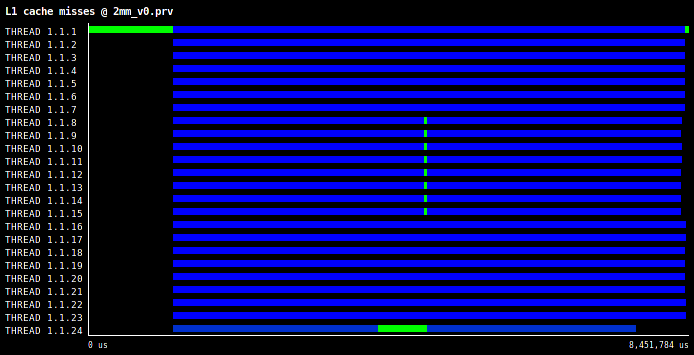
\includegraphics[width=0.99\textwidth]{figs/L1_cache_misses@2mm_v0.png}
 \end{column}
 \begin{column}{0.5\textwidth}
 \\\underline{Better locality due to tiling usage}
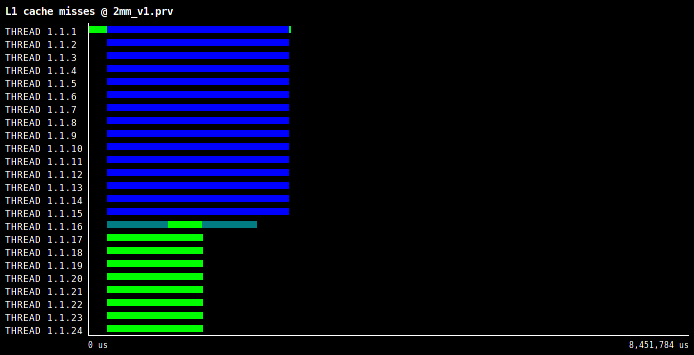
\includegraphics[width=0.99\textwidth]{figs/L1_cache_misses@2mm_v1.png}
 \end{column}
\end{columns}
\end{frame}


\begin{frame}{An example of Issue \#5 in Paraver (code05)}
Do it yourself
\begin{itemize}
    \item Connect to FT2 with X export: {\tt ssh -X youruser@ft6.cesga.es}
    \item Clone the repository: {\tt git clone https://github.com/diegoandradecanosa/extraeCoursecodes}
    \item Enter in directory code02: {\tt cd extraeCoursecodes/code03}
    \item Generate the traces (they have already been generated by me): {\tt ./generatetraces.sh}
    \item Load the paraver module:  {\tt module load paraver}
    \item Load the first trace: {\tt wxparaver 2mm\_v0.prv}
    \item Visualize using configuration counters\_papi/architecture/L1D\_misses.cfg
    \item Do the same for the other trace 2mm\_v1.prv
\end{itemize}
\end{frame}




\section{Visualization and optimization of distributed memory parallelized codes}


\begin{frame}{Distributed-memory parallelized codes}
\begin{itemize}
    \item These codes use several nodes in a supercomputer/cluster which are connected through an interconnection network
    \item One or several processes are executed on each node
    \item Each task can be itself parallelized (in shared-memory) using (for instance) OpenMP
    \item There are different libraries to exploit this kind of parallelism
        \begin{itemize}
            \item Message Passing Interface (MPI) (The most common one) \uncover<2>{\textcolor{red}{We will focus on this study case}}
            \item Unified Parallel C (UPC) and PGAS libraries and languages in general
            \item Specificic purpose libraries, such as Hadoop (for map-reduce appications) or Tensorflow (for deep learning) 
        \end{itemize}
\end{itemize}
\end{frame}

\subsection{Small intro to MPI}

\begin{frame}{Small intro to MPI}
The \emph{Message Passing Interface (MPI)}\footnote{\url{https://computing.llnl.gov/tutorials/mpi/}}  is a  message passing library standard)

The latest version of the standard is MPI 3.1 (2015)

Popular MPI implementations:
\begin{itemize}
    \item MPICH
    \item OpenMPI
    \item Intel MPI
\end{itemize}

Programming model

\centering
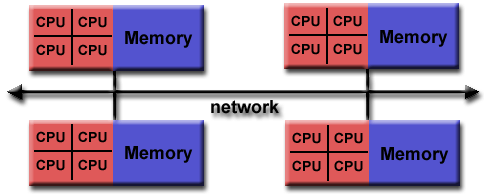
\includegraphics[width=0.7\textwidth]{figs/hybrid_mem.png}
\end{frame}

\begin{frame}{Small intro to MPI: Basics}
\begin{description}
\item[Headers] Include the MPI header using {\tt \#include <mpi.h>}
\item[Functions] In C all the MPI functions start with mpi\_
\item[Error codes] Most MPI functions includes/returns an error parameter/code. However, you won't be able to capture it as they usually break the program
\item[Groups and communications] They are MPI objects which define groups of MPI processes that can communicate to each other. {\tt MPI\_WORLD\_COMM} is the universal communicator
\item[Rank] It is the unique id of a process within a communicator
\item[Compiling] Use one of the MPI wrapper scripts of an implementation (e.g. {\tt mpicc}) to compile easily a MPI code
\item[Running] Use the mpirun/srun command to run an MPI program
\end{description}
\end{frame}

\begin{frame}{Small intro to MPI: Structure of a MPI program}
\centering
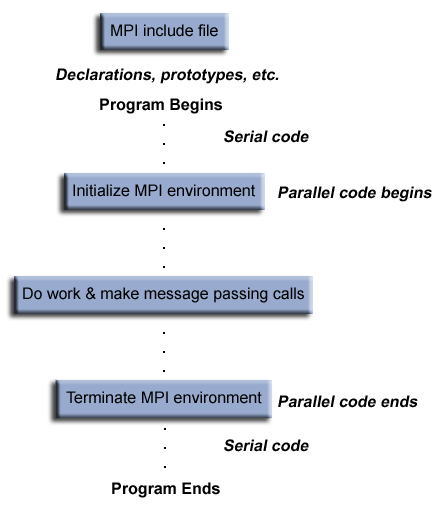
\includegraphics[width=0.5\textwidth]{figs/prog_structure.png}
\end{frame}

\begin{frame}{Small intro to MPI: Types of MPI routines}
\begin{itemize}
\footnotesize
    \item Environment management: Initialize and finalize environment, get the rank of the current process, \ldots
    \item Point to point communications: Send and receive data between a pair of nodes
        \begin{itemize}
            \item Blocks vs non-blocking routines
        \end{itemize}
    \item Collective communications: Send and receive data between groups of nodes, one to many, many to one, many to many
        \begin{itemize}
            \item Broadcast: same is data is broadcast to several processes
            \item Scatter: different pieces of data are sent to different processes
            \item Gather: different pieces of data are received from different processes
            \item Reduce: different pieces of data of different processes are combined through a given operation
        \end{itemize}
    \item (Vector) derived data types: Define special data types that can be used to encapsulate the information that is sent or received 
    \item Group \& communicator management: Create special groups and communicators
    \item Virtual topologies: Create virtual topologies that are used to arrange processes in a geometric shape
\end{itemize}
    
\end{frame}

\begin{frame}[fragile]{Small intro to MPI: Hello world}

 \begin{lstlisting}[style=C,gobble=3,caption={HelloWorld.c}]
    #include <stdio.h>
    #include <mpi.h>

    main(int argc, char **argv)
    {
        int node;
   
        MPI_Init(&argc,&argv);
        MPI_Comm_rank(MPI_COMM_WORLD, &node);
     
        printf("Hello World from Node %d\n",node);
            
        MPI_Finalize();
    }
\end{lstlisting}
\end{frame}
%Hybrid MPIOpenPM adjustment of the number of MPI processes and OpenMP thread
%Blocking vs non-blocking communication
%Exploration of different job distribution policies for the same algorithm

\subsection{Identifying MPI Performance issues with Paraver}
% Main source: https://computing.llnl.gov/tutorials/mpi_performance/#Factors

\begin{frame}{Studying a MPI trace with Paraver: Step 1 - Parallel efficiency}
Start with configuration scripts/parallel\_eficciency.cfg (Table)

\begin{columns}
\begin{column}{0.5\textwidth}
  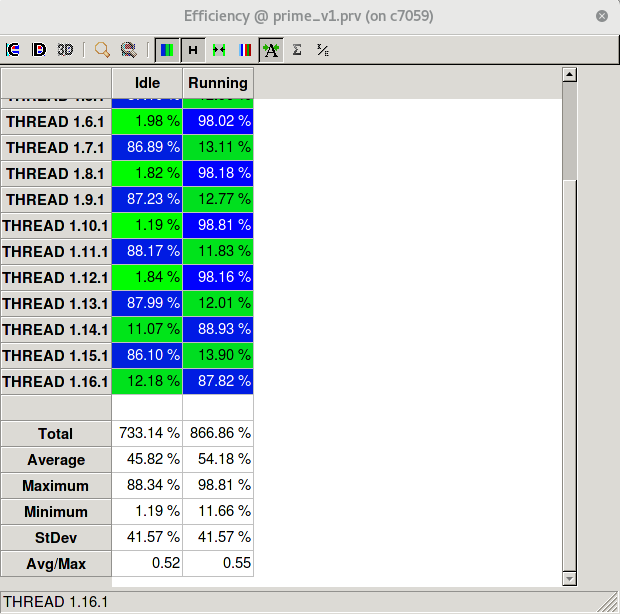
\includegraphics[width=\textwidth]{figs/parallel_efficiency_table.png}
\end{column}
\begin{column}{0.5\textwidth}
In the running column
  \begin{itemize}
      \item The average value represents parallel efficiency (the larger the better)
      \item The maximum value is the communication efficiency (the larger the better)
      \item The Avg/Max represent the load imbalance (the larger the better)
      \item This code has a heavy load imbalance
  \end{itemize}
\end{column}
\end{columns}
\end{frame}

\begin{frame}{Studying a MPI trace with Paraver: Step 1 (alt) - Useful duration}
It can be confirmed with this other configuration General/views/useful\_duration.cfg (Table)

  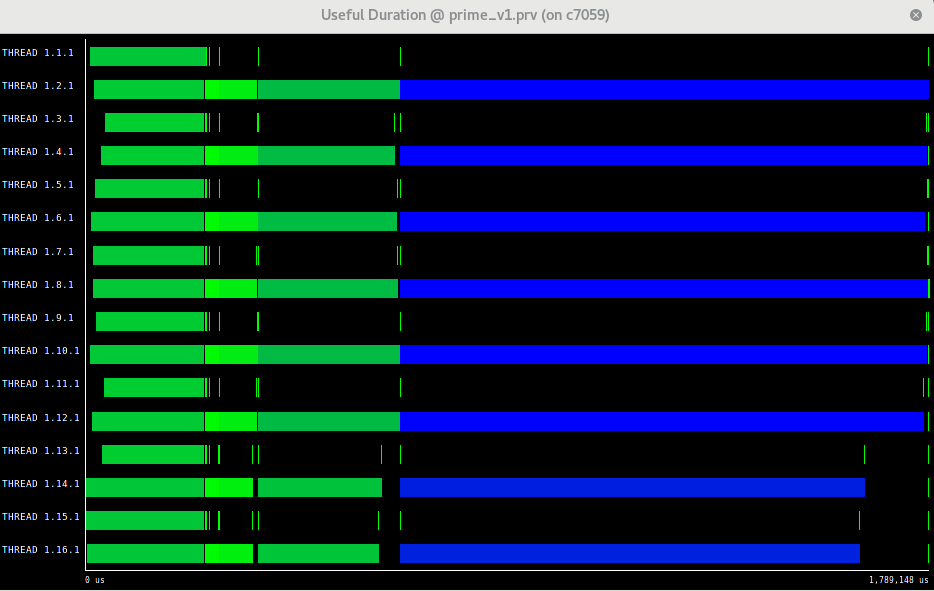
\includegraphics[width=0.6\textwidth]{figs/useful_duration_timeline.png}
  
  It shows the average duration of a computation between MPI calls
  
  The work is here clearly unbalanced (green represent much shorter values than blue)

\end{frame}

\begin{frame}{Studying a MPI trace with Paraver: Step 1 (alt) - MPI stats}
The mpi/analysis/mpi\_stats.cfg configuration show us another view of what is going on

  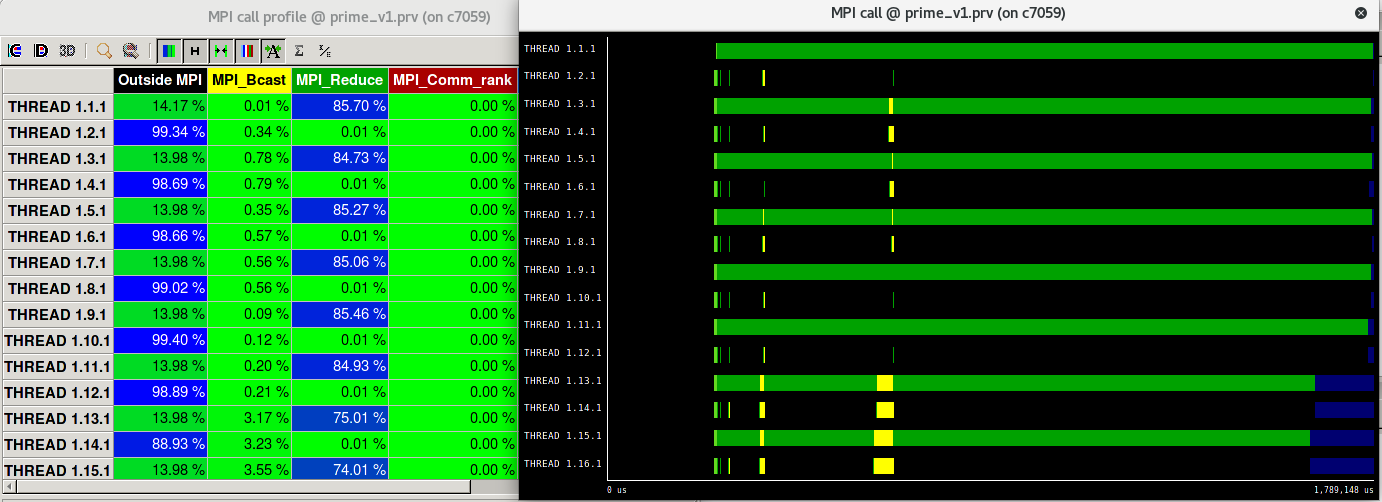
\includegraphics[width=0.8\textwidth]{figs/mpi_stats.png}

    It exists an evident load imbalance
    
\end{frame}

\begin{frame}{Studying a MPI trace with Paraver: Step 2 - IPC profile}
To identify the cause of the imbalance, we can use the IPC profile extraeCoursecodes/common/cfgs/IPC\_profile.cfg (Table)

\begin{columns}
\begin{column}{0.5\textwidth}
  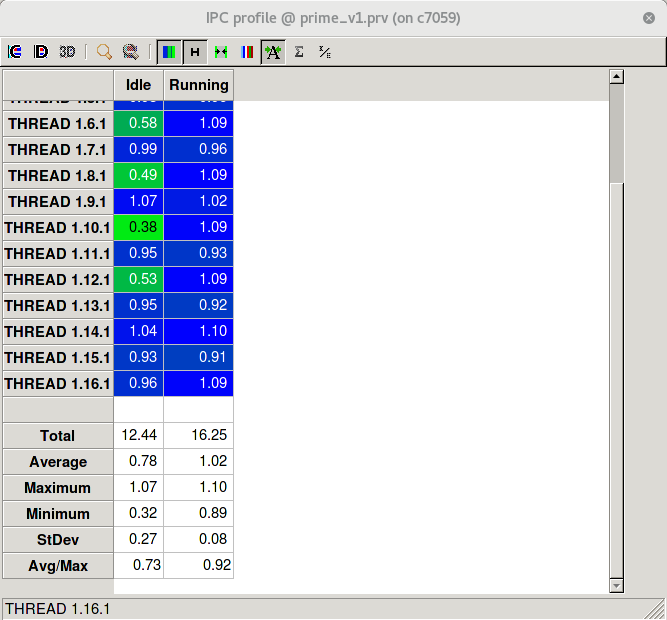
\includegraphics[width=\textwidth]{figs/ipc_profile_table.png}
\end{column}
\begin{column}{0.5\textwidth}
In the running column
  \begin{itemize}
      \item The Avg/Max is close to 1, so, this doesn't seem to be the cause
  \end{itemize}
\end{column}
\end{columns}
\end{frame}

\begin{frame}{Studying a MPI trace with Paraver: Step 2 - instructions profile}
Or we can use the instruction profile extraeCoursecodes/common/cfgs/instructions\_profile.cfg (Table)

\begin{columns}
\begin{column}{0.5\textwidth}
  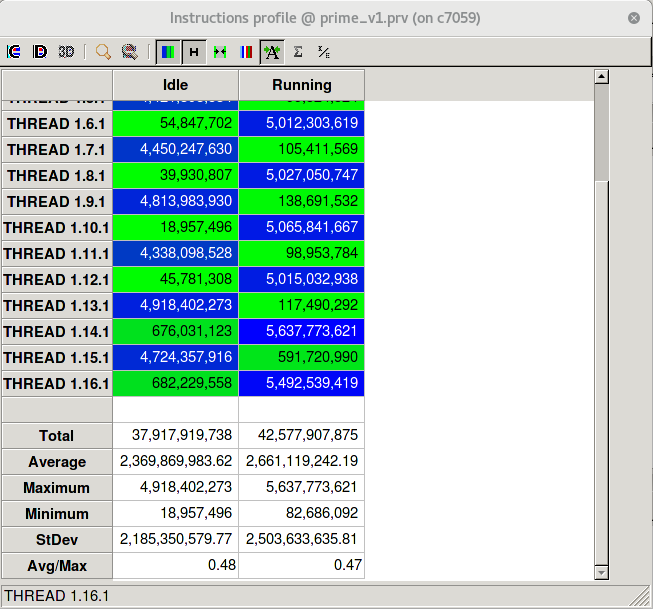
\includegraphics[width=\textwidth]{figs/ins_profile_table.png}
\end{column}
\begin{column}{0.5\textwidth}
In the running column
  \begin{itemize}
      \item The Avg/Max is  NOT close to 1, so, this  seems to be the cause
      \item Some processes are doing more job than others
  \end{itemize}
\end{column}
\end{columns}
\end{frame}


\begin{frame}{Main MPI Performance Factors}
\begin{itemize}
    \item The hardware platform of each node (CPU clock speed, cache, main memory,\ldots)
    \item The interconnection network (technology, protocol, latency, bandwidth,\ldots)
    \item \underline{The application implementation:}
        \begin{itemize}
            \item Algorithm efficiency and scalability
            \item Communication to computation ratios
            \item Load balance
            \item Serialization
            \item Memory access patterns
            \item I/O required
            \item Average message size
            \item Types of MPI routines used (blocking/non-blocking, point-to-point/collective)            
        \end{itemize}
    \item  The Performance of the MPI implementation used (message buffering, protocols, synchronization, quality of the implementation of the MPI primitives)
\end{itemize}
    
\end{frame}

\begin{frame}{Identifying serialization in Paraver}
Inspecting mpi/Poisson example: This code solves the Poisson equation in a 2D region. 

\begin{itemize}
    \item The Jacobi iterative method is used to solve the linear system
    \item The domain is divided into strips
    \item As the code is an stencil, it requires the exchange of overlapped region after each iteration
    \item The inner area of each strip can be computed in the meantime
\end{itemize}
\end{frame}

\begin{frame}{Identifying serialization in Paraver}

There are two different versions of the poisson code:

\begin{description}
\item[possion\_v0] uses blocking communications to exchange the overlapped regions
\item[possion\_v0] uses {\bf NON}-blocking communications to exchange the overlapped regions
    \begin{itemize}
        \item It allows to overlap the computation of non-overlapped regions with the communication
    \end{itemize}
\end{description}
    
\end{frame}
\begin{frame}{Identifying serialization in Paraver}
\centering
poisson\_v0\\
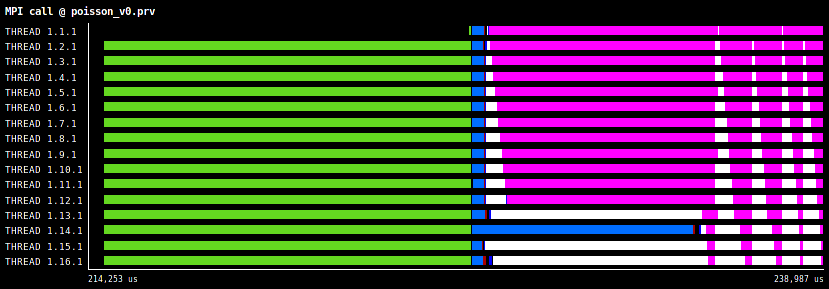
\includegraphics[width=0.8\textwidth]{figs/MPI_call@poisson_v0.png}\\
poisson\_v1\\
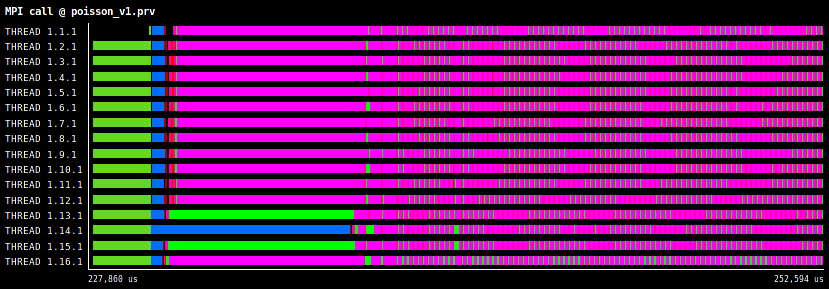
\includegraphics[width=0.8\textwidth]{figs/MPI_call@poisson_v1.png}\\
\end{frame}

\begin{frame}{Identifying load imbalance in Paraver}
Inspecting mpi/prime example: This code calculates the number of primes values until a fixed maximum. The code has several iterations where different maximums are evaluated.

Work distribution is big concern in this algorithm. The Std/Max statistic of the instructions\_profile.cfg configuration is a good metric to detect load imbalance
\begin{description}
\footnotesize
\item[prime\_v0] makes a consecutive distribution. Some processes get smaller values (with less potential divisor to be evaluated) and others get larger values. Std/Max values is 0.47 $\Rightarrow$ Load imbalance
\item[prime\_v1] makes a block-cyclic distribution. Still even values (which are categorized as non-prime soon when divided by 2) are assigned to certain processes.  Std/Max values is 0.45 $\Rightarrow$ Load imbalance
\item[prime\_v2] make a block-cyclic distribution, discarding even values by definition.  Std/Max values is 0.8 $\Rightarrow$ Better load balance
\end{description}
\end{frame}

\begin{frame}{Identifying load imbalance in Paraver}
The differences between the three versions can be clearly visualized using the mpi\_stats.cfg configuration

\centering
prime\_v0

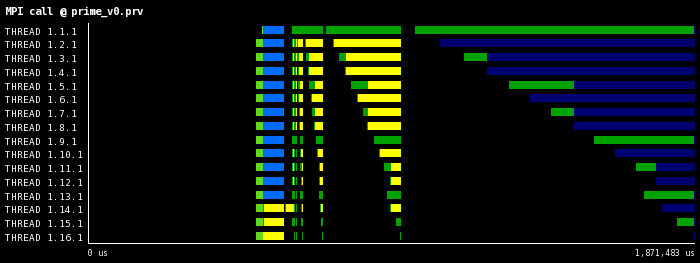
\includegraphics[width=0.8\textwidth]{figs/MPI_call@prime_v0.png}

    
\end{frame}

\begin{frame}{Identifying load imbalance in Paraver}
The differences between the three versions can be clearly visualized using the mpi\_stats.cfg configuration

\centering
prime\_v1

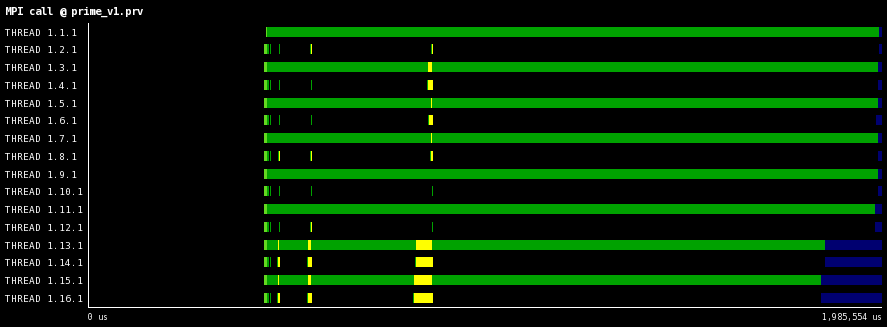
\includegraphics[width=0.8\textwidth]{figs/MPI_call@prime_v1.png}

    
\end{frame}

\begin{frame}{Identifying load imbalance in Paraver}
The differences between the three versions can be clearly visualized using the mpi\_stats.cfg configuration

\centering
prime\_v2

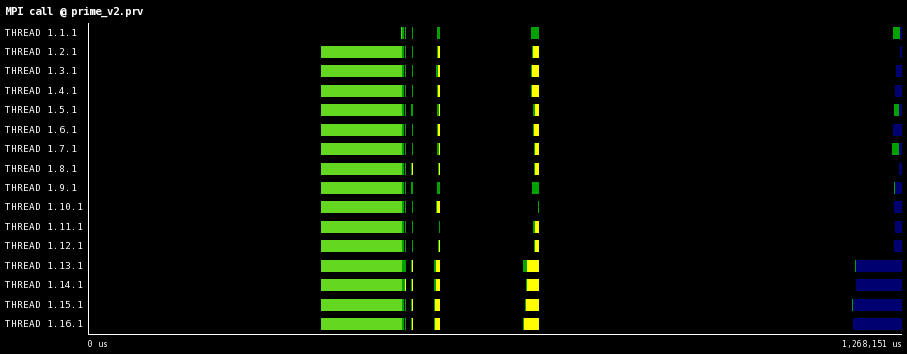
\includegraphics[width=0.8\textwidth]{figs/MPI_call@prime_v2.png}

    
\end{frame}


\begin{frame}{Hybrid applications}

The behavior of MPI+OpenMP application can also be analyzer with Extrae+Paraver.

Cardiac\_demo is an example

This is a mpi\_stats.cfg visualization using 16 MPI processes in 4 nodes and 16 OpenMP threads on each node
    
\end{frame}

\begin{frame}{Hybrid applications}

The behavior of MPI+OpenMP application can also be analyzer with Extrae+Paraver.

and this is a mpi\_stats.cfg visualization using 4 MPI processes in 4 nodes and 24 OpenMP threads on each node
    
\end{frame}

\end{document}
